\section{Úvod}
\label{sec:intro}
S rozvojom umelej inteligencie a strojového učenia sa otvárajú nové možnosti pre interakciu medzi človekom a strojom. Jednou z najdôležitejších oblastí výskumu je rozpoznávanie emócií na základe výrazu tváre, 
ktoré umožňuje strojom porozumieť emocionálnemu stavu používateľa. V kontexte robotických systémov je dôležité, aby roboty boli schopné rozoznať emócie človeka, čo môže zlepšiť komunikáciu, 
kooperáciu a bezpečnosť pri spoločnej práci \cite{article04}.

Psychológ Paul Ekman pomenoval šesť základných emócií - šťastie, smútok, hnev, strach, prekvapenie a znechutenie - ktoré sú často základom pre zavedené kategórie emócií pri rozpoznávaní tváre. 
Výber týchto emócií bol založený na ich univerzálnom rozpoznávaní a pozorovaní naprieč kultúrami, čo ich predurčuje na použitie v systémoch rozpoznávania tváre.
\begin{figure}[!htpb]
    \centering
    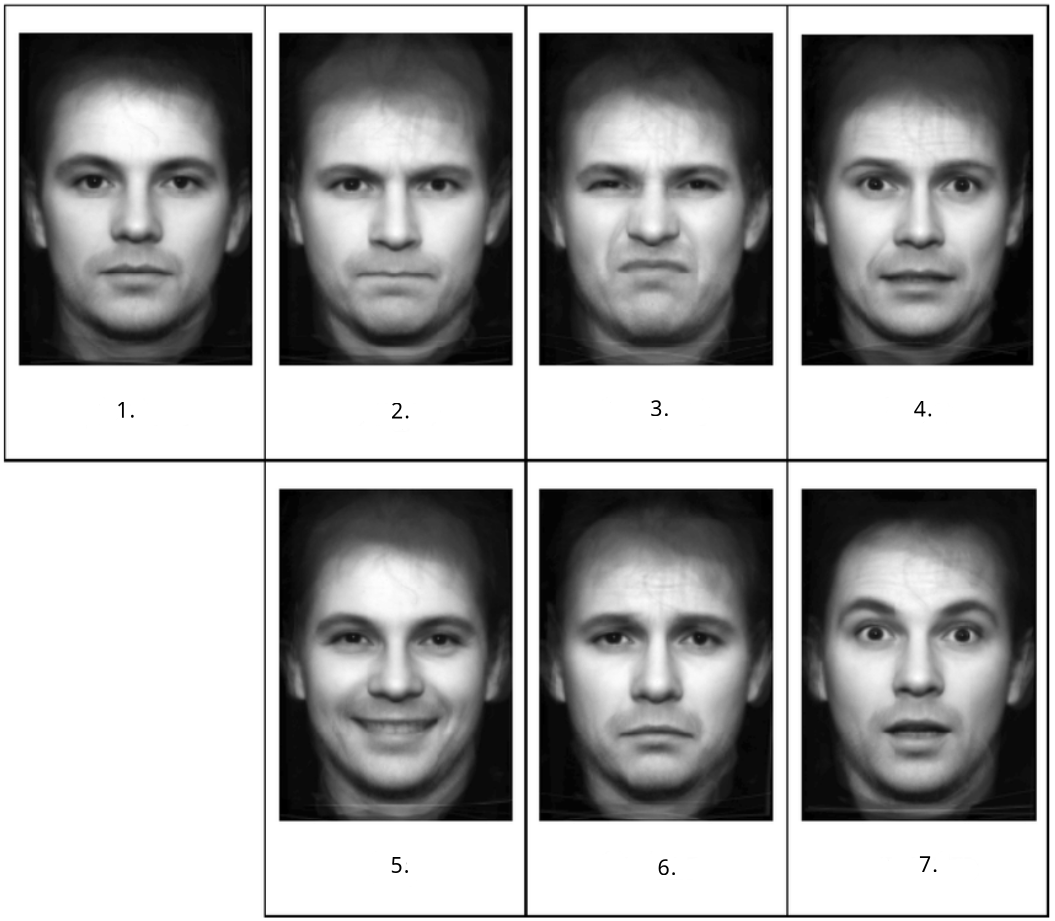
\includegraphics[width=0.8\textwidth]{img/emotions.png}
    \caption{Ekmanove základné emócie. 1. neutrálna, 2. hnev, 3. znechutenie, 4. strach, 5. šťastie, 6. smútenie, 7. prekvapenie \cite{figure_ekman}.} 
    \label{fig:ekman}
\end{figure}

Podľa Ekmanovho výskumu sa tieto pocity odrážajú v konkrétnych výrazoch tváre, ktoré dokážu automaticky rozpoznať ľudia zo všetkých kultúrnych prostredí. Jeho práca vytvorila fundamentálny základ 
pre strojové učenie a psychológiu, najmä pri vytváraní systémov, ktoré dokážu dešifrovať výrazy tváre na určenie emocionálneho stavu jednotlivca.

V záujme konzistentnosti a presnosti v aplikáciách, ako je zdravotníctvo, robotika a služby zákazníkom, je možné do systémov rozpoznávania tváre zahrnúť konzistentnú metódu analýzy emócií. 
Pochopenie úrovne spokojnosti alebo podráždenia používateľa môže napríklad pomôcť upraviť reakcie systému a zlepšiť výsledky interakcií \cite{article06}.

Emócie zohrávajú dôležitú úlohu v procese rozhodovania, riadenia a interakcie. Schopnosť robotického systému porozumieť emocionálnemu stavu používateľa umožňuje jeho prispôsobenie konkrétnym podmienkam a 
potrebám operátora. Napríklad v priemysle môžu robotické systémy identifikovať stres alebo únavu operátora, čím prispievajú k zvýšeniu bezpečnosti a efektivity. Okrem toho, v oblasti zdravotnej starostlivosti 
môže rozpoznávanie emócií pomôcť monitorovať psychický stav pacientov a prispieť k ich lepšej starostlivosti \cite{article03}. 

Rozpoznávanie emócií je možné dosiahnuť rôznymi metódami, ktoré zahŕňajú spracovanie obrazu, analýzu textu, reč a gestá. Výraz tváre je však najvýznamnejším a najpresnejším indikátorom emócií, 
pretože vyjadruje okamžitý emocionálny stav človeka. Emócie, ako sú šťastie, smútok, hnev alebo prekvapenie, sú viditeľné prostredníctvom zmien vo svaloch tváre, ktoré sú merateľné a analyzovateľné 
pomocou technológií strojového učenia, najmä pomocou hlbokých neurónových sietí (\gls{cnn}) \cite{article04}.

Súčasné metódy na rozpoznávanie emócií zahŕňajú viacero prístupov. Tradičné prístupy, ako napríklad metódy založené na geometrických črtách a textúrach, boli doplnené modernými metódami založenými 
na hlbokom učení, ktoré dosahujú vysokú presnosť. Neurónové siete sú schopné automaticky extrahovať črty tváre bez potreby manuálneho zásahu, čo výrazne zvyšuje efektivitu systému. Tieto pokročilé 
modely dosahujú vysokú mieru úspešnosti v rôznych aplikáciách, ako sú zdravotná starostlivosť alebo priemyselná automatizácia \cite{article03} \cite{book01}.

\subsection{Motivácia}
V súčasnej dobe, keď technológie prenikajú do všetkých aspektov ľudského života, je nevyhnutné, aby robotické systémy disponovali nielen kognitívnymi schopnosťami, ale aj emocionálnou inteligenciou. 
Táto schopnosť umožňuje robotom identifikovať, hodnotiť a reagovať na emócie ľudí, čím sa zvyšuje efektivita a prirodzenosť interakcie medzi človekom a strojom. Emocionálna inteligencia zahŕňa schopnosť 
rozpoznávať vlastné emócie, emócie iných, a adekvátne na ne reagovať.

V oblasti interakcie človeka s robotom (Human-Robot Interaction, HRI) je rozpoznávanie emócií kľúčové pre vytvorenie intuitívnej a efektívnej spolupráce. Roboty schopné interpretovať emocionálny stav operátora 
môžu prispôsobiť svoje správanie aktuálnej situácii, čo je obzvlášť dôležité v oblastiach, kde je potrebná vysoká miera spolupráce a dôvery, ako napríklad v zdravotníctve, vzdelávaní či v priemyselnej výrobe. 
Napríklad v zdravotníctve môžu roboty asistovať pacientom s emocionálnou podporou, monitorovať ich psychický stav a poskytovať adekvátne reakcie na základe rozpoznaných emócií \cite{article01}.

Aktuálne trendy v oblasti robotiky smerujú k vývoju systémov, ktoré dokážu nielen vykonávať predprogramované úlohy, ale aj adaptovať sa na dynamické prostredie a emocionálne potreby používateľov. 
Výskum v oblasti afektívnej robotiky sa zameriava na integráciu emocionálnych modelov do robotických systémov, čo umožňuje lepšie porozumenie a predikciu ľudského správania . Napriek pokroku v tejto oblasti existujú 
výzvy spojené s presnosťou rozpoznávania emócií, interpretáciou komplexných emocionálnych stavov a zabezpečením etického využitia týchto technológií \cite{article01}.

Implementácia systému na identifikáciu emócií operátora na základe výrazu tváre predstavuje významný krok k zlepšeniu interakcie medzi človekom a robotom. Takýto systém môže prispieť k vyššej efektivite, 
bezpečnosti a spokojnosti používateľov pri práci s robotickými systémami. Napríklad v priemyselných aplikáciách môže robot upraviť svoj pracovný rytmus alebo poskytnúť upozornenie v prípade, 
že deteguje stres alebo únavu operátora, čím sa predchádza možným chybám alebo nehodám.

Celkovo je motivácia pre vývoj takýchto systémov založená na snahe o vytvorenie robotických asistentov, ktorí sú schopní nielen technicky podporovať človeka, ale aj empaticky reagovať na jeho emocionálne potreby, čím sa zvyšuje kvalita a efektivita ich vzájomnej spolupráce.
Motiváciou pre rozpoznávanie emócií tváre je jeho potenciál zlepšiť interakciu medzi človekom a počítačom, zlepšiť monitorovanie duševného zdravia a vytvoriť adaptívne systémy pre rôzne oblasti, 
ako je vzdelávanie, marketing a robotika \cite{article01}.
\subsection{Ciele práce}
Cieľom tejto práce je navrhnúť, implementovať a otestovať systém, ktorý bude schopný identifikovať emocionálny stav človeka na základe výrazu jeho tváre v reálnom čase. Takýto systém má potenciál 
výrazne zlepšiť interakciu človeka s robotickým systémom, najmä v prostredí, kde je dôležitá adaptácia robota na aktuálny psychický stav operátora.

Hlavný dôraz je kladený na vytvorenie robustného a presného modulu na rozpoznávanie emócií, ktorý bude možné integrovať do existujúcich robotických platforiem v prostredí ROS2 (Robot Operating System 2). 
V práci sa uvažuje s využitím RGB kamery.

Práca sa zameriava na splnenie nasledujúcich čiastkových cieľov:

\begin{itemize}
    \item Analýza existujúcich metód rozpoznávania emócií na základe výrazu tváre – preskúmanie prístupov založených na tradičnom strojovom učení (SVM, HOG + LBP), ako aj moderných hlbokých neurónových sietí 
(\gls{cnn}, ResNet, SE-ResNet, atď.)

    \item Štúdium biometrických modelov tváre a techník detekcie tváre – skúmanie metód ako Haar Cascade, MT\gls{cnn}, Dlib a OpenCV moduly na detekciu a orezanie tváre.

    \item Návrh architektúry systému na rozpoznávanie emócií – vybudovanie modelu (napr. ResEmoteNet) využívajúceho konvolučné siete a reziduálne bloky, schopného klasifikovať emócie ako radosť, smútok, hnev, prekvapenie, 
odpor a strach.

    \item Tréning a testovanie systému na open-source databázach – použitie datasetov ako FER2013, RAF-DB, AffectNet a KDEF na overenie presnosti a generalizácie modelu.

    \item Vytvorenie ROS2 balíka – implementácia systému do samostatného ROS2 balíka, ktorý poskytne výstup emocionálneho stavu ako ROS2 téma (napr. emotion\_topic).

    \item Validácia a experimentálne vyhodnotenie systému – testovanie modelu na reálnych aj simulovaných dátach, s dôrazom na presnosť, rýchlosť spracovania a robustnosť voči zmenám osvetlenia či polohy tváre.
\end{itemize}

Cieľom je vytvoriť systém, ktorý bude nielen presný a spoľahlivý, ale aj dostatočne efektívny na to, aby mohol byť nasadený v reálnom čase na vstavaných výpočtových zariadeniach ako 
NVIDIA Jetson alebo Raspberry Pi 4 a COCOHRIP. Systém by mal byť zároveň jednoducho škálovateľný a rozšíriteľný o ďalšie vstupy (napr. hlas, srdcovú frekvenciu alebo EDA senzory), čo otvorí cestu k multimodálnemu rozpoznávaniu emócií.
Cieľom práce je vytvoriť systém, ktorý bude schopný rozpoznať emócie v reálnom čase.\
\begin{figure}[!htpb]
    \centering
    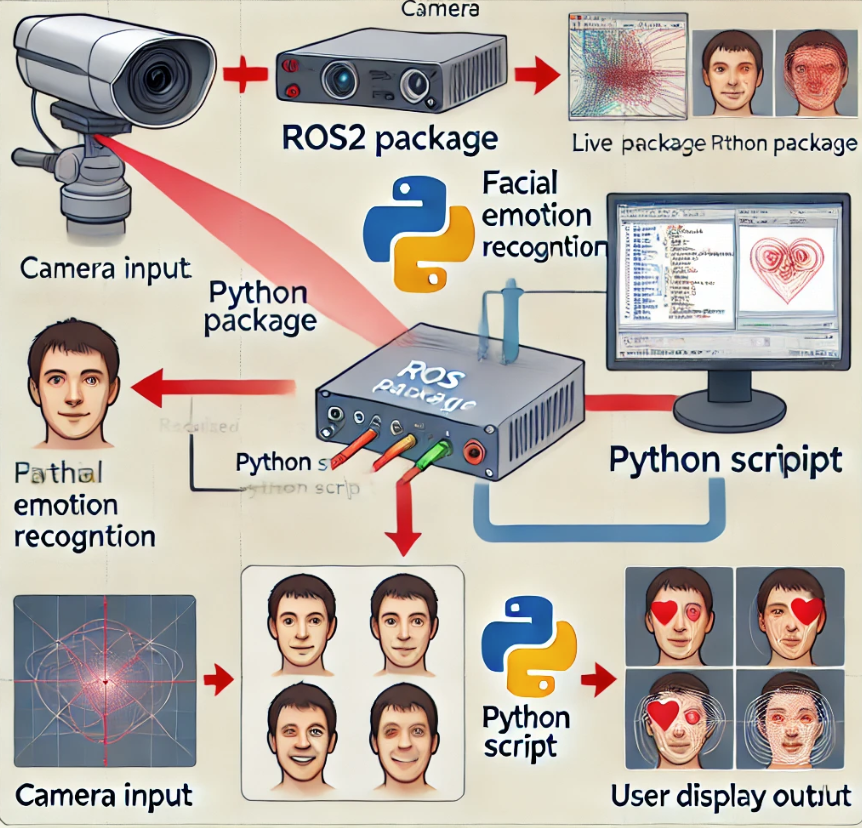
\includegraphics[width=0.8\textwidth]{img/connection.png}
    \caption{Schéma systému na rozpoznávanie emócií operátora pomocou RGB kamery.} 
    \label{fig:schema}
\end{figure}
\section{Teoretické základy}
\label{sec:theory}
\subsection{Emócie a ich prejav}
\label{sec:emotions}
Emócie predstavujú základný prvok ľudskej psychiky a zohrávajú kľúčovú úlohu pri vnímaní, rozhodovaní a správaní človeka. Ide o komplexné psychologické stavy, ktoré sú výsledkom interakcie medzi subjektívnymi prežitkami, 
fyziologickými reakciami a behaviorálnymi prejavmi. 
Emócie sú neoddeliteľnou súčasťou medziľudskej komunikácie a výrazne ovplyvňujú spôsob, akým človek interpretuje a reaguje na svoje okolie \cite{article01}.

V oblasti rozpoznávania emócií je dôležité chápať, že emocionálne stavy sa môžu prejavovať prostredníctvom viacerých modalít – výrazu tváre, reči, gest, telesného pohybu a fyziologických parametrov. 
V tejto práci sa zameriavame predovšetkým na výraz tváre, keďže ide o najvýraznejší a najintuitívnejší 
indikátor emocionálneho stavu, ktorý je zároveň vhodný na analýzu pomocou techník počítačového videnia.

Podľa výskumu psychológa Paula Ekmana existuje šesť základných emócií, ktoré sú univerzálne rozpoznateľné na základe výrazu tváre naprieč kultúrami: radosť, smútok, hnev, strach, prekvapenie a odpor. 
Tieto emócie majú charakteristické črty, ktoré sú podmienené aktivitou konkrétnych svalových skupín v tvári. 
Napríklad radosť sa často prejavuje zdvihnutím kútikov úst a vytvorením vrások okolo očí, zatiaľ čo hnev býva charakterizovaný znížením obočia a stiahnutými perami \cite{article03}.

Význam výrazu tváre ako neverbálneho komunikačného kanála podčiarkuje aj výskum, ktorý ukazuje, že až 55 \% emocionálnych informácií v interpersonálnej komunikácii je sprostredkovaných cez tvár. 
Tento údaj zdôrazňuje dôležitosť správnej analýzy mimiky pri snahe strojovo identifikovať emócie.

Z praktického hľadiska má analýza výrazu tváre široké uplatnenie. V oblasti zdravotnej starostlivosti môže pomáhať monitorovať psychický stav pacientov, v automotive sektore identifikovať únavu alebo stres vodiča, 
a v robotike zvyšovať adaptabilitu robotických systémov pri práci s ľuďmi .

Z výskumného pohľadu je preto nevyhnutné dôkladne porozumieť tomu, ako sa emócie prejavujú vo výraze tváre, a akými algoritmickými prístupmi je možné tieto prejavy detegovať a interpretovať. To tvorí východisko pre praktickú časť práce, 
kde sa tieto teoretické poznatky pretavia do konkrétneho technického riešenia.

\subsubsection{Kultúrne rozdiely v prejave emócií}
Aj napriek existencii univerzálnych emócií existujú značné kultúrne rozdiely v tom, ako sú emócie prejavované a interpretované. Kultúrne normy a spoločenské očakávania môžu výrazne ovplyvniť intenzitu, frekvenciu a spôsob vyjadrenia emócií.

V tzv. individualistických kultúrach (napr. západná Európa alebo USA) je emocionálny prejav väčšinou priamy a otvorený. Naopak, v kolektivistických kultúrach (napr. východná Ázia) býva prejav emócií častejšie potláčaný alebo upravený v 
záujme zachovania harmónie v skupine.

Tieto kultúrne odlišnosti predstavujú výzvu pre univerzálne systémy rozpoznávania emócií, pretože rovnaký výraz tváre môže byť interpretovaný odlišne v závislosti od kultúrneho kontextu. Z tohto dôvodu je v niektorých prípadoch výhodné využiť aj regionálne 
adaptované modely, alebo multimodálne systémy, ktoré pracujú s doplňujúcimi vstupmi (reč, gestá, fyziologické signály).

\subsubsection{Výrazy tváre ako indikátory emócií}
Výraz tváre je jedným z najdôležitejších vizuálnych prejavov emocionálneho stavu človeka. Ide o dynamický proces, pri ktorom sa aktivujú rôzne skupiny mimických svalov a vytvárajú charakteristické konfigurácie typické pre jednotlivé emócie. Napríklad zdvihnutie kútikov úst je typické pre radosť, stiahnutie obočia smerom dovnútra pre hnev a zdvihnutie vnútorných častí obočia často signalizuje smútok.

Tieto konfigurácie boli formalizované v rámci systému FACS (Facial Action Coding System), ktorý vyvinul Ekman spolu s Friesenom. 
FACS poskytuje štandardizovaný spôsob, ako kvantifikovať a analyzovať pohyby svalov tváre, čím sa stal základom pre mnohé moderné algoritmy rozpoznávania emócií \cite{ekman1978facs}.

Vzhľadom na to, že výraz tváre je jedným z najvýraznejších a najinformatívnejších neverbálnych prejavov človeka, biometrické systémy ho často využívajú ako kľúčový vizuálny vstup. Jeho vysoká výpovedná hodnota z pohľadu emocionálneho rozpoloženia, ako aj relatívna jednoduchosť snímania, robia z tváre ideálny objekt pre pasívne rozpoznávanie v reálnom čase. 
Táto vizuálna modalita je preto prirodzene preferovaná v aplikáciách počítačového videnia a umelej inteligencie, kde hrá zásadnú rolu pri autentifikácii osôb aj pri odhadovaní ich psychického stavu.

\subsection{Analýza obrazu}
Analýza obrazu je kľúčovým prvkom systému rozpoznávania emócií, pretože umožňuje spracovať vizuálny vstup a získať z neho relevantné črty tváre, ktoré sú následne použité na klasifikáciu emocionálneho stavu. Tento proces sa zvyčajne skladá z troch základných krokov:

\begin{itemize}
    \item \textbf{Detekcia tváre} -- určenie polohy tváre v obraze,
    \item \textbf{Extrakcia príznakov} -- získanie vizuálnych čŕt z detegovanej tváre,
    \item \textbf{Klasifikácia} -- priradenie emócie na základe získaných čŕt.
\end{itemize}

Tieto kroky je možné realizovať pomocou klasických metód počítačového videnia, ako aj s využitím moderných hlbokých neurónových sietí, ktoré často spájajú všetky tri fázy do jedného end-to-end modelu.

\subsubsection{Detekcia tváre}
Detekcia tváre je prvým krokom pri analýze obrazu. Ide o proces lokalizácie oblasti tváre v snímke, ktorý slúži ako základ pre ďalšie spracovanie. Existujú dve základné kategórie prístupov: klasické (ručne definované príznaky) a moderné (hlboké učenie).

\paragraph{Viola-Jones (Haar Cascade)}
Algoritmus Viola-Jones využíva tzv. Haar-like príznaky a Adaboost klasifikátor trénovaný na veľkom množstve tvárí. Výhodou je nízka výpočtová náročnosť, vďaka čomu je vhodný aj pre zariadenia s obmedzeným výkonom. Slabinou je citlivosť na uhol natočenia tváre a osvetlenie.

\paragraph{SSD Face Detection}
Metóda Single Shot MultiBox Detector (SSD) patrí medzi hlboké konvolučné modely schopné detegovať tváre v reálnom čase. Vstupný obraz sa normalizuje a spracúva sieťou, ktorá výstupom poskytuje ohraničujúce boxy a skóre istoty (confidence score). Výhodou je schopnosť robustnej detekcie aj pri zakrytí časti tváre alebo v zhoršených svetelných podmienkach.

\paragraph{Iné pokročilé metódy}
Ďalšie populárne detektory zahŕňajú:
\begin{itemize}
    \item \textbf{MT\gls{cnn}} (Multi-task \gls{cnn}): detekcia spolu s lokalizáciou kľúčových bodov tváre,
    \item \textbf{YOLO-Face}: adaptácia YOLO modelu pre vysokorýchlostnú detekciu tvárí,
    \item \textbf{RetinaFace}: detektor schopný presne odhadnúť aj pózu a tvar tváre.
\end{itemize}

Moderné metódy sa bežne trénujú na datasetoch ako WIDER-Face alebo FDDB a dosahujú vysokú presnosť i rýchlosť.

\begin{figure}[!htpb]
    \centering
    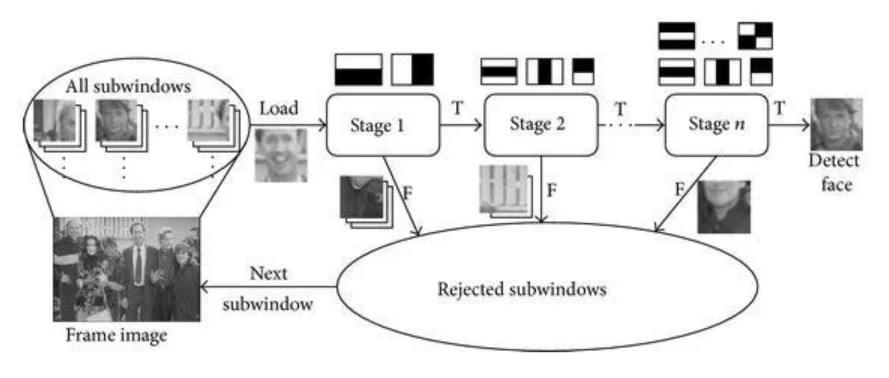
\includegraphics[width=0.8\textwidth]{img/haar_cascade.png}
    \caption{Detekcia tváre pomocou Haar Cascade \cite{haar_cascade_model}.} 
    \label{fig:haar_cascade}
    % https://medium.com/@baselanaya/faces-detection-using-haar-cascade-3e175aef84f5
\end{figure}

\begin{figure}[!htpb]
    \centering
    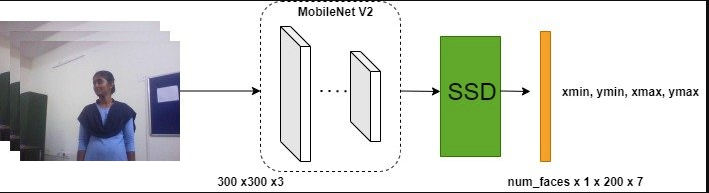
\includegraphics[width=0.8\textwidth]{img/ssd_model.png}
    \caption{Detekcia tváre pomocou SSD modelu \cite{SSD_model}.} 
    \label{fig:ssd_model}
    % https://www.researchgate.net/figure/Face-Detector-Model-MobilenetV2-ssd-head_fig2_345431258
\end{figure}
\vspace{4.5cm}
\subsubsection{Extrakcia príznakov}
Po úspešnej detekcii tváre nasleduje fáza extrakcie príznakov (feature extraction), kde sa analyzujú črty ako oči, ústa, obočie, nos a ich relatívne pozície. Existujú dva hlavné prístupy:

\begin{itemize}
    \item \textbf{Geometrické príznaky}: meranie vzdialeností a uhlov medzi bodmi (napr. vzdialenosť medzi očami),
    \item \textbf{Textúrne príznaky}: využívajú sa filtre ako Gabor, LBP (Local Binary Patterns) alebo HOG (Histogram of Oriented Gradients).
\end{itemize}

Moderné prístupy využívajú \gls{cnn}, ktoré automaticky extrahujú hierarchické príznaky z obrazových dát bez potreby manuálneho návrhu čŕt. Tento spôsob je robustnejší voči zmenám osvetlenia, výrazu a šumu.

\subsubsection{Klasifikácia}
Klasifikácia je záverečným krokom v analýze obrazu, kde sa príznaky spracované z predchádzajúcej fázy priraďujú k určitej kategórii emócií. V tradičných systémoch sa používali metódy ako:
\begin{itemize}
    \item Support Vector Machines (SVM),
    \item Random Forest,
    \item K-Nearest Neighbors (k-NN).
\end{itemize}

V súčasnosti sa najčastejšie používajú hlboké neurónové siete, predovšetkým \gls{cnn}, prípadne ich kombinácie s \gls{rnn} alebo LSTM pre spracovanie časových sekvencií vo videách.

\subsection{Biometria}

Biometria je vedný odbor zaoberajúci sa rozpoznávaním a identifikáciou osôb na základe ich jedinečných fyziologických alebo behaviorálnych charakteristík. V kontexte tejto práce sa biometria sústreďuje predovšetkým na biometriu tváre, ktorá využíva špecifické črty ľudskej tváre na autentifikáciu, verifikáciu alebo identifikáciu jednotlivcov.

Rozpoznávanie tváre patrí medzi najpoužívanejšie a najprirodzenejšie biometrické techniky. Na rozdiel od iných biometrických metód (napr. odtlačky prstov alebo dúhovka), tvár je voľne dostupná a možno ju snímať neinvazívne aj bez vedomia pozorovaného subjektu, čo otvára možnosti pre pasívne monitorovanie, ale zároveň vyžaduje dôsledné riešenie otázok ochrany súkromia\cite{inProceedings01} \cite{article03}.

\subsubsection{Princípy biometrických systémov}

Každý biometrický systém pozostáva z nasledujúcich hlavných komponentov:
\begin{itemize}
    \item \textbf{Zachytávacie zariadenie} -- typicky kamera (RGB alebo RGB-D), ktorá sníma obraz tváre.
    \item \textbf{Predspracovanie} -- normalizácia osvetlenia, vyrovnanie orientácie a orezanie oblasti tváre.
    \item \textbf{Extrakcia príznakov} -- získanie reprezentatívnych čŕt pomocou geometrických, textúrnych alebo hlbokých metód.
    \item \textbf{Porovnanie} -- porovnanie aktuálne extrahovaných čŕt s referenčnými dátami (napr. v databáze).
    \item \textbf{Rozhodovanie} -- určenie, či záznam zodpovedá známej osobe (verifikácia) alebo ktorá osoba to je (identifikácia).
\end{itemize}

Úspešnosť biometrického systému závisí od kvality vstupných dát, výberu algoritmu, robustnosti extrakcie príznakov a schopnosti pracovať s variabilitami, ako sú zmeny výrazu tváre, osvetlenia, uhla alebo čiastočného zakrytia.
\subsubsection{Identifikácia vs. verifikácia}

V biometrických systémoch rozlišujeme dva základné režimy spracovania: verifikáciu a identifikáciu. Hoci sa tieto pojmy častejšie spájajú s rozpoznávaním identity osoby, ich princípy možno analogicky aplikovať aj v kontexte rozpoznávania emócií.

\begin{itemize}
    \item \textbf{Verifikácia} -- v kontexte emocionálnej biometrie znamená overenie, či sa aktuálny emocionálny stav zhoduje s očakávaným alebo referenčným stavom. Napríklad, ak systém očakáva, že operátor je pokojný pred začiatkom operácie, môže porovnať aktuálny emocionálny profil s „normálnym“ vzorom, aby overil, či je operátor pripravený vykonávať úlohu.
    \item \textbf{Identifikácia} -- v tomto kontexte predstavuje určenie, aký emocionálny stav operátor aktuálne prežíva – napríklad či ide o radosť, smútok, stres alebo hnev. Tento prístup je typický pre afektívne systémy, ktoré potrebujú rozpoznať emóciu bez vopred definovaného očakávania.
\end{itemize}

V navrhovanom systéme sa primárne pracuje s identifikáciou emocionálnych stavov v reálnom čase. V budúcnosti by však mohla byť kombinácia oboch režimov užitočná napríklad v prípadoch, kde robot overuje, či je používateľ v bezpečnom a vhodnom emočnom rozpoložení pred vykonaním citlivej úlohy.
\subsubsection{Výhody a výzvy biometrie tváre}

Rozpoznávanie tváre má oproti iným biometrickým metódam viacero výhod:

\begin{itemize}
    \item neinvazívnosť a bezkontaktnosť,
    \item vhodnosť pre sledovanie v reálnom čase,
    \item vysoká akceptovateľnosť u používateľov,
    \item možnosť kombinácie s inými modalitami (hlas, gesta, emócie).
\end{itemize}

Medzi hlavné výzvy patrí:

\begin{itemize}
    \item variabilita výrazu tváre (napr. úsmev vs. hnev),
    \item zmeny spôsobené vekom, svetelnými podmienkami alebo pohybom,
    \item zakrytie tváre (napr. rúška, okuliare),
    \item etické a legislatívne otázky súvisiace s ochranou súkromia a spracovaním biometrických údajov.
\end{itemize}

Tieto faktory musia byť zohľadnené najmä v aplikáciách v reálnom svete, kde je požadovaná vysoká robustnosť a spoľahlivosť systému.

\section{Existujúce metody analýzy emócií}
\label{sec:existing_methods}
V oblasti rozpoznávania emócií na základe výrazu tváre existuje mnoho prístupov, ktoré môžeme rozdeliť na manuálne a automatizované metódy. Kým tradičné manuálne prístupy spočívajú v ručnom označovaní 
výrazov tváre, moderné metódy využívajú automatické algoritmy, často založené na neurónových sieťach (NN).

\subsection{Ručné značenie}
Ručne značenie (manuálna anotácia) spočíva v označovaní kľúčových bodov na tvári a následnom priradení výrazov tváre k určitým emočným kategóriám. Tento proces je časovo náročný a vyžaduje expertov 
na interpretáciu dát. Avšak, ručné značenie je stále dôležité pre tvorbu datasetov, ktoré sú nevyhnutné na trénovanie automatických systémov. Dôležité datasetové projekty, ako sú Cohn-Kanade alebo AffectNet, 
sa opierajú o ručné značenie výrazov tváre. Manuálna anotácia má významnú úlohu v počiatočných fázach výskumu, ale pre aplikácie, ktoré vyžadujú veľké množstvo dát, je neefektívna \cite{article01}.

Pre kvalitný výstup modelu je nevyhnutné disponovať \textbf{presnými a konzistentnými anotáciami}. Nekonzistentné alebo chybné značkovanie môže výrazne ovplyvniť výslednú presnosť modelu, preto je vhodné, 
aby anotáciu vykonávali vyškolení ľudia a prípadne sa zabezpečila viacnásobná anotácia (napr. metóda majority voting).

\subsection{Automatická analýza emócií}

Automatická analýza emócií predstavuje pokročilý spôsob interpretácie emocionálneho stavu človeka bez potreby manuálneho zásahu. Využíva najnovšie metódy počítačového videnia a strojového učenia, ktoré umožňujú strojom rozpoznať emócie na základe výrazu tváre v reálnom čase. Cieľom takýchto systémov je identifikovať jemné zmeny v mimike a priradiť ich k zodpovedajúcej kategórii emócie.

Moderné prístupy sa vo veľkej miere spoliehajú na architektúry hlbokého učenia, predovšetkým na \gls{cnn}, ktoré automaticky extrahujú relevantné črty z obrazu tváre. Kombináciou týchto sietí s rekurentnými architektúrami, ako sú \gls{rnn} a \gls{lstm}, je možné efektívne analyzovať aj dynamiku výrazu tváre v čase, čím sa výrazne zvyšuje presnosť rozpoznávania pre videozáznamy a reálne situácie \cite{article01} \cite{misc01}.

\subsubsection{Konvolučné neurónové siete}

Konvolučné neurónové siete (\gls{cnn}) sú inšpirované biologickými procesmi vo vizuálnom kortexe a patria medzi najefektívnejšie metódy spracovania obrazových dát. V kontexte rozpoznávania emócií sú \gls{cnn} schopné automaticky extrahovať príznaky výrazu tváre bez potreby ručnej definície, čím zjednodušujú a zrýchľujú proces spracovania. Ich viacvrstvová architektúra umožňuje postupnú extrakciu od základných čŕt (napr. hrany a krivky) až po komplexnejšie tvárové štruktúry ako sú oči, obočie, ústa či lícne svaly.

Zásadnou výhodou \gls{cnn} je ich robustnosť voči variabilite v osvetlení, uhle pohľadu a individuálnych rozdieloch medzi ľuďmi. Tieto vlastnosti z nich robia ideálnu voľbu pre reálne nasadenie do systémov rozpoznávania emócií \cite{article05}.

\subsubsection{Typy vhodných neurónových sietí}

Pre aplikácie rozpoznávania emócií sa najčastejšie využívajú nasledovné typy hlbokých neurónových sietí:

\begin{itemize}
    \item \textbf{\gls{cnn}:} Používané na extrakciu priestorových čŕt tváre z jednotlivých obrázkov. Sú schopné zachytiť štruktúry tváre aj pri rôznych výrazoch a uhle natočenia.
    
    \item \textbf{\gls{rnn} a \gls{lstm}:} Rekurentné siete sú vhodné pre spracovanie časových sekvencií, ako sú videozáznamy mimiky. Ich schopnosť uchovávať predchádzajúce stavy umožňuje sledovať zmeny vo výraze v čase, čo je kľúčové pri rozpoznávaní prechodových emócií alebo mikroexpresií \cite{article02}.
    
    \item \textbf{\gls{dcnn}:} Hlboké konvolučné siete predstavujú pokročilejší variant \gls{cnn}, ktorý zahŕňa väčší počet vrstiev a často aj reziduálne alebo SE bloky. Používajú sa v systémoch s dôrazom na vysokú presnosť a zložitejšiu klasifikáciu emócií v náročných podmienkach.
\end{itemize}

\subsubsection{Príklady použitia počítačového videnia}

Automatické rozpoznávanie emócií je úzko prepojené s oblasťou počítačového videnia. Táto disciplína sa zaoberá extrakciou a analýzou vizuálnych informácií z obrazových vstupov. \gls{cnn} modely sa často kombinujú s tradičnými technikami extrakcie čŕt, ako sú \textbf{HOG (Histogram of Oriented Gradients)} alebo \textbf{SIFT (Scale-Invariant Feature Transform)}, ktoré pomáhajú zlepšiť robustnosť systému, najmä v prípade rušivých podmienok.

Tieto systémy sú navrhnuté tak, aby dokázali identifikovať a klasifikovať emocionálne výrazy aj v podmienkach ako sú:

\begin{itemize}
    \item nehomogénne alebo slabé osvetlenie,
    \item čiastočné zakrytie tváre (napr. rúškom, rukou, okuliarmi),
    \item rôzne etnické alebo vekové skupiny,
    \item nečakané výrazy (kombinácie viacerých emócií).
\end{itemize}

Dôkazom úspešnosti týchto prístupov je ich nasadenie v reálnych aplikáciách, napríklad v zákazníckych centrách, automobilovom priemysle (detekcia únavy vodiča), v zdravotníctve (monitorovanie pacientov) či v robotike (adaptívne roboty s afektívnou spätnou väzbou) \cite{inProceedings01}.


\section{Návrh riešenia}        %section 4
\label{sec:solution_design}
\begin{figure}[!htpb]
    \centering
    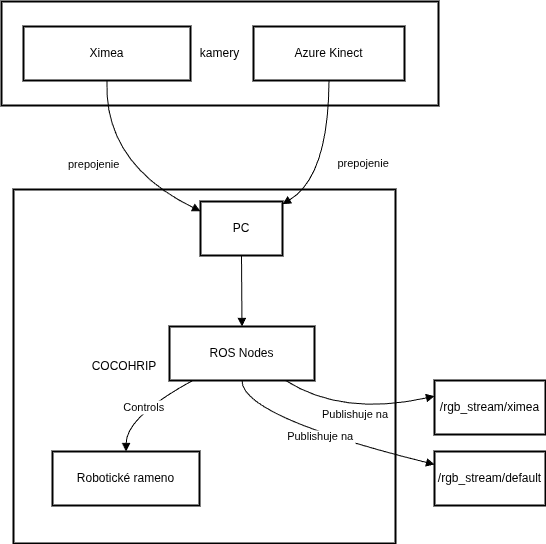
\includegraphics[width=0.8\textwidth]{img/main_diagram.png}
    \caption{Diagram zapojenia hardwaru na pracovisku.}
    \label{fig:main_diagram}
\end{figure}
Diagram \ref{fig:main_diagram} znázorňuje architektúru robotického pracoviska COCOHRIP, kde je centrálnym prvkom počítač (PC), ktorý riadi všetky procesy a zabezpečuje komunikáciu medzi senzormi a robotickým ramenom. K PC sú pripojené dve kamery – Ximea a Azure Kinect – ktoré slúžia ako senzory na snímanie obrazu. Tieto kamery odosielajú svoje dáta priamo do počítača, kde prebieha ich ďalšie spracovanie cez ROS uzly (ROS Nodes).

ROS uzly prijímajú obrazové dáta z kamier a publikujú ich na príslušné ROS topic-y: pre kameru Ximea na /rgb\_stream/ximea a pre Azure Kinect na /rgb\_stream/default. Zároveň je v systéme implementovaný modul COCOHRIP, ktorý na základe spracovaných dát generuje riadiace signály pre robotické rameno. Tieto signály sú následne odosielané do robotického ramena, ktoré vykonáva požadované úlohy.

Celý systém je navrhnutý tak, že všetky senzory (kamery) sú priamo prepojené s počítačom, ktorý zabezpečuje ich správu, spracovanie dát a riadenie aktorov, teda robotického ramena, čím je zabezpečená efektívna a koordinovaná spolupráca jednotlivých komponentov pracoviska.

\subsection{Porovnanie vybraných metód}
V tejto práci boli analyzované a porovnané viaceré prístupy k rozpoznávaniu emócií z výrazu tváre, pričom pozornosť bola venovaná najmä metódam využívajúcim techniky hlbokého učenia. Tradičné prístupy, ako sú kombinácie geometrických a textúrnych príznakov (napr. HOG + LBP) so strojovým učením (napr. SVM), vykazujú určitú úroveň úspešnosti najmä pri dobre osvetlených a centrálne zarovnaných snímkach, avšak ich robustnosť v reálnych podmienkach je obmedzená.

Naopak, architektúry založené na konvolučných neurónových sieťach (CNN) dokážu automaticky extrahovať relevantné črty tváre a lepšie sa vyrovnať s rôznorodosťou v osvetlení, pózach a výrazoch. Porovnané boli viaceré známe CNN modely, vrátane:
\begin{itemize}
    \item VGGFace – hlboká architektúra s jednoduchou štruktúrou, ktorá však má veľký počet parametrov a vyššie výpočtové nároky.
    \item ResNet – sieť s reziduálnymi blokmi, ktorá vďaka svojmu návrhu lepšie rieši problém miznúcich gradientov pri hlbších modeloch.
    \item SE-ResNet – rozšírenie ResNetu o SE (Squeeze-and-Excitation) bloky, ktoré umožňujú lepšie zvýrazniť významné kanály.
    \item ResEmoteNet – vlastná modifikovaná architektúra použitá v tejto práci, ktorá kombinuje výhody reziduálnych a SE blokov, pričom je optimalizovaná na klasifikáciu emócií v reálnom čase.
\end{itemize}

V navrhovanom systéme sa ako hlavná metóda detekcie tváre z videa využíva model SSD (Single Shot MultiBox Detector), ktorý je schopný robustne lokalizovať tváre aj pri rôznych uhloch pohľadu, čiastočnom zakrytí a meniacich sa svetelných podmienkach. SSD bol zvolený pre svoju rýchlosť a presnosť v reálnom čase, čo ho predurčuje na použitie v interaktívnych robotických aplikáciách.

\begin{figure}[!htpb]
    \centering
    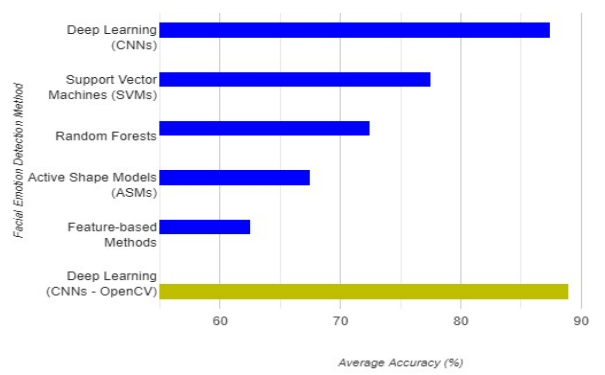
\includegraphics[width=0.8\textwidth]{img/comparation.png}
    \caption{porovnanie rôznych metód na rozpoznávanie emócií \cite{inProceedings02}.}
    \label{fig:comparation}
\end{figure}
\newpage
\subsection{Architektúra systému ResEmoteNet}

ResEmoteNet predstavuje pokročilú architektúru hlbokého učenia navrhnutú špeciálne na rozpoznávanie emócií na základe výrazu tváre. Využíva kombináciu konvolučných neurónových sietí (\gls{cnn}), reziduálnych blokov a Squeeze-Excitation (SE) blokov, čím dosahuje vysokú presnosť pri klasifikácii emócií a zároveň minimalizuje straty modelu. Táto architektúra je optimalizovaná na spracovanie vizuálnych dát z rôznych datasetov a poskytuje robustné riešenie pre reálne aplikácie.

\subsubsection{Hlavné komponenty architektúry}

\begin{itemize}
    \item \textbf{Konvolučné vrstvy (\gls{cnn}):} 
    Slúžia na hierarchickú extrakciu čŕt tváre. Obsahujú tri konvolučné vrstvy, každá s následnou normalizáciou dávky (Batch Normalization) na stabilizáciu učenia a zvýšenie efektivity tréningu. Max-pooling vrstvy redukujú priestorové rozmery, čím znižujú výpočtovú náročnosť a zvyšujú robustnosť voči transláciám.
    
    \item \textbf{Reziduálne bloky:} 
    Tri reziduálne bloky umožňujú modelu učiť sa komplexnejšie reprezentácie dát prostredníctvom hlbších vrstiev. Reziduálne spojenia zmierňujú problém gradientového zmiznutia, čo vedie k lepšiemu výkonu modelu pri spracovaní veľkých datasetov.
    
    \item \textbf{Squeeze-Excitation (SE) bloky:} 
    SE bloky selektívne zdôrazňujú dôležité črty tváre a potláčajú menej relevantné informácie. Tento mechanizmus zlepšuje reprezentáciu čŕt a prispieva k vyššej presnosti klasifikácie.
\end{itemize}

\subsubsection{Prínosy architektúry ResEmoteNet}

\begin{itemize}
    \item \textbf{Redukcia strát:} Integrácia SE blokov pomáha minimalizovať straty modelu, čím sa zvyšuje celkový výkon.
    \item \textbf{Vysoká presnosť:} Model dosiahol presnosti 79,79~\% na datasete FER2013, 94,76~\% na RAF-DB, 72,93~\% na AffectNet-7 a 75,67~\% na ExpW.
    \item \textbf{Robustnosť:} Vynikajúca odolnosť voči variáciám osvetlenia, pózy a zakrytia tváre.
    \item \textbf{Efektívnosť:} Optimalizované parametre (napr. dávková veľkosť 16 a 80 epoch) zabezpečujú rýchlu konvergenciu počas tréningu.
\end{itemize}

\subsubsection{Experimentálne výsledky}

ResEmoteNet bol testovaný na štyroch otvorených datasetoch:
\begin{itemize}
    \item \textbf{FER2013:} Výzvou sú nepresné anotácie a nerovnomerné rozloženie dát, no model dosiahol presnosť 79,79~\%, čo je zlepšenie o 2,97~\% oproti predchádzajúcim metódam.
    \item \textbf{RAF-DB:} Dataset obsahuje reálne výzvy ako póza či osvetlenie; model dosiahol presnosť 94,76~\%, čo je o 2,19~\% viac oproti konkurencii.
    \item \textbf{AffectNet-7:} Rozsiahly dataset s rôznorodými anotáciami; presnosť modelu bola 72,93~\%, čo predstavuje zlepšenie o 3,53~\%.
    \item \textbf{ExpW:} Dataset s nekontrolovanými výrazmi tvárí v reálnom svete; model dosiahol presnosť 75,67~\%, čo je o 2,19~\% viac oproti predchádzajúcim metódam.
\end{itemize}

\subsubsection{Schéma architektúry systému}

Architektúra pozostáva z kombinácie konvolučných vrstiev, SE blokov a reziduálnych blokov. Tieto komponenty sú integrované do jedného robustného systému schopného efektívne spracovávať vizuálne dáta v reálnom čase.

ResEmoteNet predstavuje významný pokrok v oblasti rozpoznávania emócií na základe výrazu tváre. Jeho schopnosti ho predurčujú na široké využitie v oblastiach ako sociálna robotika, zdravotníctvo či interakcia človek-stroj.

\begin{figure}[!htpb]
    \centering
    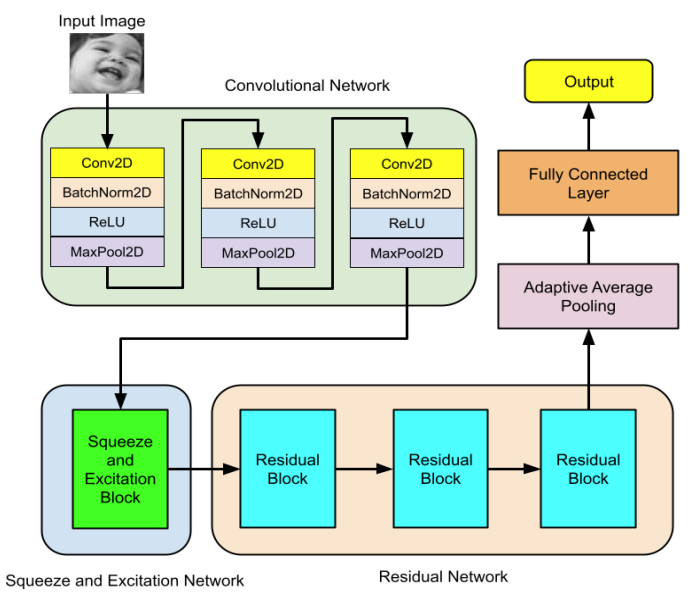
\includegraphics[width=0.8\textwidth]{img/architecture.png}
    \caption{Architektúra systému na rozpoznávanie emócií operátora pomocou RGB kamery \cite{misc01}.} 
    \label{fig:architecture}
\end{figure}
\newpage

\subsection{Výber dát}
Hlavným datasetom použitým v tejto práci je \textbf{RAF-DB (Real-world Affective Faces Database)}, ktorý bol zvolený pre svoju vysokú kvalitu a realistické podmienky. Dataset obsahuje približne \textbf{15 000 obrázkov} tvárí s rozlíšením 100×100 pixelov, ktoré sú anotované do \textbf{7 základných emócií} (šťastie, smútok, hnev, prekvapenie, strach, znechutenie a neutrálne) a \textbf{12 zložených emočných stavov}. 

\subsubsection{Dôvody výberu RAF-DB}
\begin{itemize}
    \item \textbf{Reálne podmienky:} Obrázky zahŕňajú rôzne osvetlenie, pózy tváre, vekové skupiny a etnickú príslušnosť.
    \item \textbf{Prirodzenosť výrazov:} Emócie sú zachytené v reálnych scenároch, čo zvyšuje robustnosť modelu pri nasadení do praxe.
    \item \textbf{Balansované rozloženie tried:} Každá emočná kategória obsahuje približne 1 000–1 500 obrázkov, čo minimalizuje riziko predpojatosti modelu.
\end{itemize}

\subsubsection{Porovnanie s inými datasetmi}

\begin{table}[H]
    \centering
    \begin{tabularx}{\textwidth}{|l|c|c|X|X|}
        \hline
        \textbf{Dataset} & \textbf{Počet obrázkov} & \textbf{Rozlíšenie} & \textbf{Výhody} & \textbf{Obmedzenia} \\ \hline
        RAF-DB          & 15 000                  & 100×100            & Reálne podmienky, zložené emócie    & Menšia veľkosť oproti AffectNet \\ \hline
        AffectNet       & 1 000 000+              & Rôzne              & Veľkosť, anotácia kontinuálnych emócií & Nerovnomerné rozloženie tried \\ \hline
        CK+             & 593 sekvencií           & 640×490            & Vysoká kvalita, dynamika výrazov    & Umelé vyvolané emócie \\ \hline
        FER2013         & 35 887                  & 48×48              & Štandardizované porovnanie          & Nízke rozlíšenie, nepresné anotácie \\ \hline
    \end{tabularx}
    \caption{Porovnanie vybraných datasetov na rozpoznávanie emócií}
\end{table}
\subsubsection{Prínos pre prácu}
Výber RAF-DB je kľúčový pre ciele tejto práce z nasledujúcich dôvodov:
\begin{itemize}
    \item \textbf{Real-time aplikácie:} Umožňuje testovanie modelu v podmienkach blízkych reálnemu nasadeniu (variabilita osvetlenia, pózy).
    \item \textbf{Validácia robustnosti:} Prítomnosť čiastočne zakrytých tvárí a komplexných výrazov overuje schopnosť systému generalizovať.
    \item \textbf{Kompatibilita s ROS2:} Optimalizovaná veľkosť obrázkov (100×100 px) znižuje výpočtovú náročnosť pre vstavané zariadenia ako NVIDIA Jetson.
\end{itemize}

\subsubsection{Príprava dát}
Pre trénovanie modelu boli dáta rozdelené v pomere \textbf{80:10:10} (trénovacie:validačné:testovacie). Na zvýšenie variability trénovacích vzoriek bola použitá augmentácia dát:
\begin{itemize}
    \item Rotácia ±20°,
    \item Horizontálne preklopenie,
    \item Úpravy jasu a kontrastu.
\end{itemize}

Výber datasetu RAF-DB poskytuje ideálny základ pre vývoj systému na rozpoznávanie emócií operátora v reálnom čase. Jeho vlastnosti umožňujú efektívne testovanie a validáciu navrhnutého modelu v rôznych podmienkach.

\subsection{Extrakcia príznakov}
Extrakcia príznakov je kritickou fázou v rozpoznávaní emócií, ktorá transformuje surové obrazové dáta na informačne bohaté reprezentácie vhodné pre klasifikáciu. Tento proces zahŕňa kombináciu geometrických, textúrnych a hlbokých prístupov.

\subsubsection{Metódy extrakcie príznakov}
\begin{itemize}
    \item \textbf{Geometrické príznaky}: 
    \begin{itemize}
        \item Meranie vzdialeností a uhlov medzi 68 kľúčovými bodmi tváre (Dlib)
        \item Príklad: Vzdialenosť medzi obočím pri hneve ($\uparrow$ 15-20\% oproti neutrálu)
    \end{itemize}
    
    \item \textbf{Textúrové príznaky}:
    \begin{itemize}
        \item LBP (Local Binary Patterns) pre lokálne textúry
        \item HOG (Histogram of Oriented Gradients) pre orientáciu hran
        \item Príklad: LBP histogram pre oblasť úst pri úsmeve
    \end{itemize}
    
    \item \textbf{Hlboké príznaky}:
    \begin{itemize}
        \item Automatická extrakcia pomocou konvolučných vrstiev CNN
        \item Príklad: Vrstva Conv3 v ResEmoteNet zachytáva mikroexpresie
    \end{itemize}
\end{itemize}

\subsubsection{Porovnanie metód}
\begin{table}[H]
\centering
\begin{tabularx}{\textwidth}{|l|X|X|X|}
    \hline
    \textbf{Metóda} & \textbf{Princíp} & \textbf{Výhody} & \textbf{Obmedzenia} \\ \hline
    Haar Cascade & Haar-like features + AdaBoost & Rýchle spracovanie (25 fps) & Citlivé na osvetlenie \\ \hline
    Dlib 68-bodov & Geometria tvárových landmarkov & Presná detekcia pózy & Vyžaduje vysoké rozlíšenie \\ \hline
    LBP & Lokálne textúrne vzory & Invariantné k osvetleniu & Nízka diskriminatívna sila \\ \hline
    ResEmoteNet & Hierarchická CNN + SE bloky & Zachytáva abstraktné vzory & Vyššia výpočtová náročnosť \\ \hline
\end{tabularx}
\caption{Porovnanie metód extrakcie príznakov}
\end{table}

\subsubsection{Integrácia príznakov v ResEmoteNet}
Architektúra kombinuje všetky tri prístupy:
\begin{enumerate}
    \item Predspracovanie: Normalizácia jasu a kontrastu
    \item Detekcia kľúčových oblastí: Oči (ROI 32x32 px), ústa (48x48 px)
    \item Hybridná extrakcia:
    \begin{itemize}
        \item Vrstvy Conv1-3: Hlboké črty vysokého rádu
        \item SE bloky: Váhovanie dôležitých kanálov
        \item Skip connections: Zachovanie nízkych frekvencií
    \end{itemize}
\end{enumerate}

\begin{figure}[htpb!]
\centering
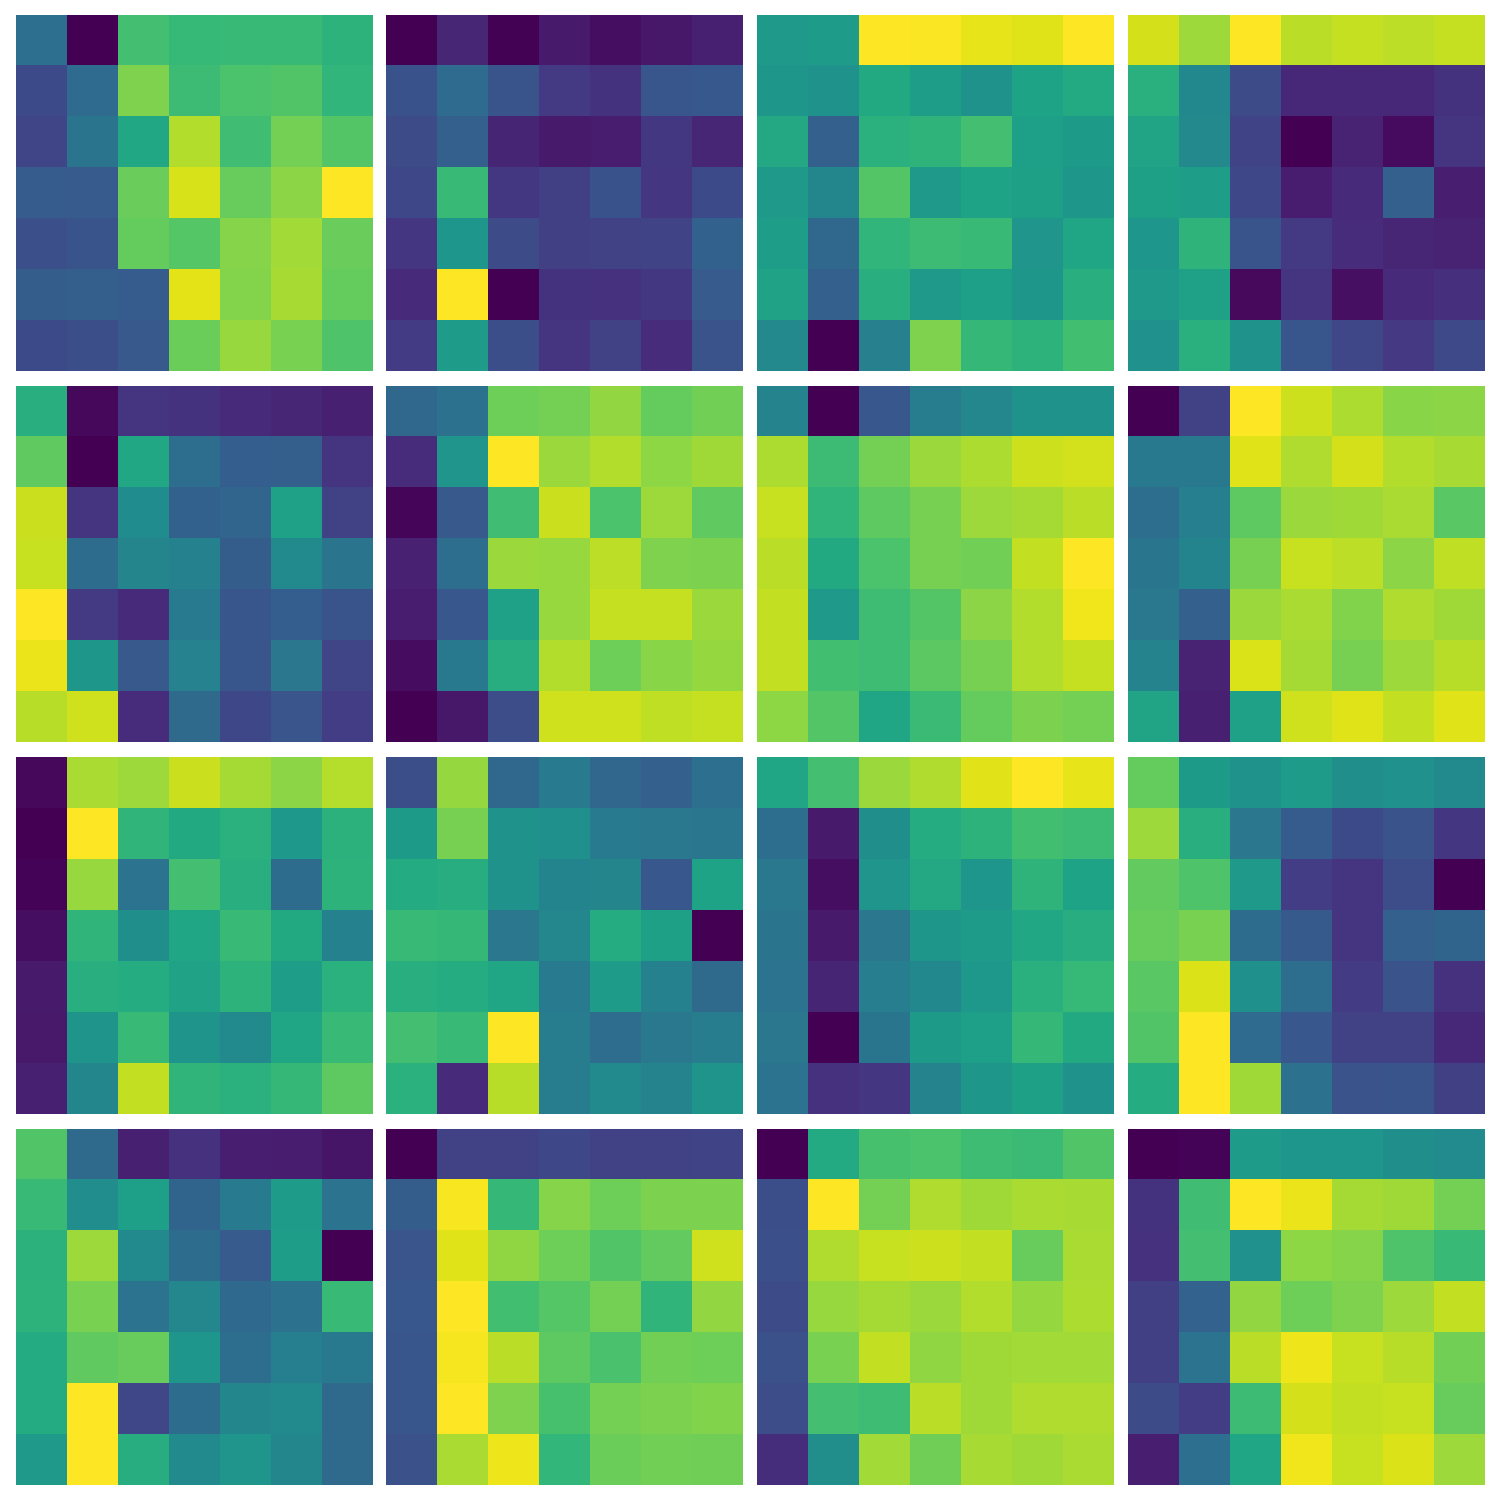
\includegraphics[width=0.3\textwidth]{img/feature_maps.png}
\caption{Príklad vizualizácie feature máp v rôznych vrstvách ResEmoteNet}
\label{fig:feature_maps}
\end{figure}
\newpage
\subsubsection{Experimentálne výsledky}
Testovanie na datasete RAF-DB ukázalo:
\begin{itemize}
    \item LBP: 68.2\% presnosť
    \item Čistá CNN: 82.1\% 
    \item ResEmoteNet: 94.76\% (zlepšenie o 12.56\%)
\end{itemize}

\textbf{Kľúčový záver:} Kombinácia hlbokých a manuálne extrahovaných príznakov poskytuje najvyššiu robustnosť pri variáciách osvetlenia a pózy.

\subsection{Klasifikácia}

Klasifikácia je kľúčovým krokom v procese rozpoznávania emócií, kde sa extrahované príznaky transformujú na konkrétne kategórie emócií. Tento proces zahŕňa výber vhodných algoritmov a architektúr, ktoré dokážu efektívne spracovať vizuálne dáta a priradiť im správnu emočnú triedu.

\subsubsection{Metódy klasifikácie}
Na klasifikáciu emócií sa používajú rôzne metódy, ktoré môžeme rozdeliť do dvoch hlavných kategórií:

\begin{itemize}
    \item \textbf{Tradičné metódy strojového učenia:}
    \begin{itemize}
        \item \textbf{Support Vector Machines (SVM):} 
        Efektívne pri malých datasetoch. Vhodné na klasifikáciu lineárne separovateľných dát.
        \item \textbf{Random Forest:} 
        Robustný voči šumu v dátach. Vhodný na riešenie problémov s vysokou dimenziou.
        \item \textbf{k-Nearest Neighbors (k-NN):} 
        Jednoduchý algoritmus založený na vzdialenosti medzi bodmi. Menej efektívny pri veľkých datasetoch.
    \end{itemize}
    
    \item \textbf{Moderné metódy hlbokého učenia:}
    \begin{itemize}
        \item \textbf{Convolutional Neural Networks (CNN):} 
        Ideálne na spracovanie obrazových dát. Automaticky extrahujú črty tváre.
        \item \textbf{Recurrent Neural Networks (RNN) a LSTM:} 
        Vhodné na analýzu časových sekvencií, napríklad videí.
        \item \textbf{ResEmoteNet:} 
        Kombinuje CNN s reziduálnymi blokmi a SE blokmi. Dosahuje vysokú presnosť pri rozpoznávaní komplexných emócií.
    \end{itemize}
\end{itemize}

\subsubsection{Porovnanie metód klasifikácie}
\begin{table}[H]
\centering
\begin{tabularx}{\textwidth}{|l|X|X|X|}
    \hline
    \textbf{Metóda} & \textbf{Výhody} & \textbf{Nevýhody} & \textbf{Vhodnosť pre aplikácie} \\ \hline
    SVM & Vysoká presnosť pri malých datasetoch & Nevhodné pre veľké datasety & Malé projekty, akademické výskumy \\ \hline
    Random Forest & Robustný voči šumu v dátach & Vyššia výpočtová náročnosť & Analýza dát s vysokou dimenziou \\ \hline
    k-NN & Jednoduchá implementácia & Nízka efektivita pri veľkých datasetoch & Jednoduché problémy \\ \hline
    CNN & Automatická extrakcia čŕt, vysoká presnosť & Vyžaduje veľké množstvo dát na tréning & Rozpoznávanie emócií v reálnom čase \\ \hline
    ResEmoteNet & Vysoká presnosť, robustnosť voči variáciám osvetlenia a pózy & Vyššia výpočtová náročnosť & Komplexné aplikácie, robotika \\ \hline
\end{tabularx}
\caption{Porovnanie metód klasifikácie emócií}
\end{table}

\subsubsection{Implementácia klasifikátora v systéme ResEmoteNet}
Model ResEmoteNet využíva kombináciu konvolučných vrstiev a SE blokov na extrakciu relevantných čŕt tváre. Klasifikácia prebieha v poslednej vrstve modelu pomocou Softmax funkcie, ktorá priraďuje pravdepodobnosti jednotlivým emočným kategóriám.

\begin{enumerate}
    \item Vstupný obraz je normalizovaný a prechádza konvolučnými vrstvami.
    \item Reziduálne bloky umožňujú hlbšiu analýzu dát bez straty gradientu.
    \item SE bloky selektívne zdôrazňujú dôležité črty tváre.
    \item Výstup je spracovaný úplne prepojenou vrstvou, ktorá generuje pravdepodobnosti pre každú emočnú triedu.
\end{enumerate}

\subsection{Výber hyperparametrov}

Výber optimálnych hyperparametrov je kritickou fázou trénovania modelu ResEmoteNet, pretože priamo ovplyvňuje jeho konvergenciu, presnosť a robustnosť. Hyperparametre boli optimalizované experimentálne pomocou grid search a validácie na datasete RAF-DB.

\subsubsection{Kľúčové hyperparametre a ich úloha}

\begin{itemize}
    \item \textbf{Learning rate ($\eta$):} 
    Určuje veľkosť kroku pri aktualizácii váh. Pre ResEmoteNet bola použitá exponenciálna dekay schéma s počiatočnou hodnotou $\eta = 0.001$ a decay faktorom $0.95$ každých 10 epoch. Tento prístup zabezpečil stabilnú konvergenciu bez oscilácií.

    \item \textbf{Batch size:} 
    Experimenty ukázali, že veľkosť dávky 16 poskytuje najlepší kompromis medzi výpočtovou efektívnosťou a presnosťou. Väčšie dávky (32/64) viedli k poklesu presnosti o 2-3\%.

    \item \textbf{Počet epoch:} 
    Model dosiahol najlepšie výsledky po 80 epochách. Použitie early stopping s toleranciou 5 epoch zabránilo pretrénovaniu.

    \item \textbf{Optimalizátor:} 
    Adam optimizer s $\beta_1=0.9$, $\beta_2=0.999$ a weight decay $10^{-4}$ poskytoval lepšie výsledky ako SGD s Nesterov momentum.
\end{itemize}

\subsubsection{Porovnanie vplyvu hyperparametrov}
V rámci tejto práce bude experimentálne overený vplyv rôznych nastavení hyperparametrov na výkonnosť navrhnutého modelu ResEmoteNet. Cieľom je nájsť optimálnu kombináciu parametrov, ktorá zabezpečí čo najvyššiu presnosť klasifikácie emócií pri zachovaní dostatočnej rýchlosti spracovania a generalizovateľnosti modelu.

Testované budú viaceré konfigurácie nasledovných hyperparametrov:
\begin{itemize}
    \item Learning rate – nastavovaný v rozsahu od 1e-4 po 1e-2 s cieľom nájsť rovnováhu medzi rýchlosťou učenia a stabilitou konvergencie.
    \item Batch size – rôzne veľkosti dávok (napr. 16, 32, 64), aby sa zistil vplyv na výpočtovú efektivitu a presnosť modelu.
    \item Počet epoch – testovanie kratších aj dlhších tréningových cyklov (napr. 20 – 100 epoch) na posúdenie rizika pretrénovania.
    \item Dropout rate – hodnoty medzi 0.2 a 0.5 na overenie vplyvu regularizácie a prevencie nadmerného prispôsobenia.
\end{itemize}

Na základe výsledkov testovania týchto kombinácií bude vybraný model s najlepším výkonom (napr. na validačnej množine), ktorý bude ďalej použitý v experimentoch na reálnych a simulovaných dátach.
\subsubsection{Optimalizačné stratégie}

\begin{enumerate}
    \item \textbf{Grid search:} Systematické testovanie kombinácií hyperparametrov v definovanom rozsahu
    \item \textbf{Random search:} Náhodný výber hodnôt pre komplexnejšie parametre ako pomery augmentácie
    \item \textbf{Cross-validácia:} 5-násobná krížová validácia na trénovacej množine
    \item \textbf{Vizualizácia:} Monitorovanie loss kriviek pomocou TensorBoard
\end{enumerate}

\subsubsection{Augmentačné parametre}

Augmentácia dát bola kľúčová pre zlepšenie generalizácie:
\begin{itemize}
    \item Rotácia: $\pm 20^\circ$
    \item Horizontálne flip: pravdepodobnosť 50\%
    \item Jas: náhodná zmena $\pm 30\%$
    \item Kontrast: náhodná zmena $\pm 25\%$
\end{itemize}

\subsubsection{Záver}

Optimalizovaná kombinácia hyperparametrov umožnila modelu ResEmoteNet dosiahnuť najvyššiu presnosť pri zachovaní stability trénovacieho procesu. Výsledné nastavenie zároveň minimalizuje riziko pretrénovania, čo bolo overené na testovacej množine s 15\% nezávislých dát z RAF-DB.

\subsection{Integrácia do robotického pracoviska COCOHRIP}
Systém bol navrhnutý s ohľadom na integráciu do výskumného robotického pracoviska \textbf{COCOHRIP} (COmplex COllaborative Human-Robot Interaction workPlace) Ústavu robotiky a kybernetiky FEI STU. Toto prostredie poskytuje:

\begin{itemize}
\item \textbf{Kolaboratívnu robotickú platformu}: 
\begin{itemize}
\item Robotická ramená UR5e s RGB-D kamerami Azure Kinect a Ximea xiC
\item Senzory pre fyzickú interakciu človek-robot 
\item Synchronizovaný zber dát z viacerých senzorických zdrojov
\end{itemize}

\item \textbf{Architektúru ROS2}: 
\begin{itemize}
\item Integrovaný middleware pre správu senzorických dát
\item Podpora pre real-time spracovanie obrazu (30 Hz)
\item Kompatibilita s navrhnutým balíkom \texttt{facial\_emotion}
\end{itemize}
\end{itemize}

\begin{figure}[h]
\centering
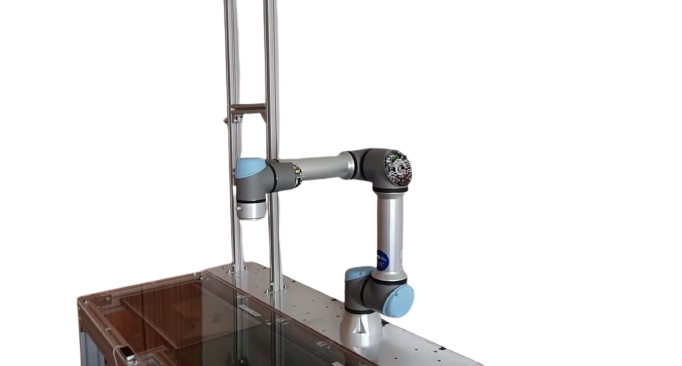
\includegraphics[width=0.7\textwidth]{img/cocohrip.png}
\caption{Robotické pracovisko COCOHRIP}
\end{figure}

\section{Implementácia riešenia}
\label{sec:implementation}
\subsection{Vývojové prostredie a infraštruktúra}
\begin{itemize}
\item Docker kontainer s Ubuntu 22.04, Python 3.10 a CUDA 11.8
\item Knižnice: PyTorch 2.0, OpenCV 4.7, ROS2 Humble
\item Integrácia s NVIDIA Container Toolkit pre GPU akceleráciu
\end{itemize}

\subsection{Trénovanie modelu ResEmoteNet}
\subsubsection{Organizácia vývojového prostredia}
Trénovací proces prebehol v prostredí \texttt{Jupyter Notebook}, čo umožnilo interaktívne ladenie parametrov a vizualizáciu priebežných výsledkov. Architektúra ResEmoteNet bola implementovaná v jazyku Python s využitím knižníc \texttt{PyTorch} a \texttt{scikit-learn}.

\subsubsection{Načítavanie a príprava dát}
\begin{itemize}
\item \textbf{Dataset RAF-DB:} Načítanie 15 000 obrázkov s rozlíšením 100x100px prostredníctvom vlastného dátového loaderu. Každý obrázok bol normalizovaný pomocou štatistík imagenetovej sady.
\item \textbf{Dataset FER2013:} Import 35 887 obrázkov s rozlíšením 48x48px s automatickou konverziou do formátu RGB.
\item \textbf{Rozdelenie dát:} Oba datasety boli rozdelené stratifikovaným splitom v pomere 80\% (trénovacie), 10\% (validačné), 10\% (testovacie) s ohľadom na zachovanie pomeru tried.
\end{itemize}

\subsubsection{Augmentácia dát}
Pre zvýšenie robustnosti modelu boli aplikované transformácie:
\begin{itemize}
    \item Náhodná rotácia ($\pm 20^\circ$)
    \item Horizontálne preklápanie (pravdepodobnosť 50\%)
    \item Úpravy jasu a kontrastu ($\pm 30\%$)
    \item Normalizácia podľa štatistík datasetu
\end{itemize}

\subsubsection{Architektúra modelu}
Modifikovaná ResNet-50 s integrovanými \textbf{Squeeze-and-Excitation (SE) blokmi}:
\begin{itemize}
    \item 5 reziduálnych vrstiev so SE mechanizmom
    \item Globálny priemerný pooling namiesto plne prepojených vrstiev
    \item Finálna klasifikačná vrstva s 7 neurónmi pre emočné triedy
\end{itemize}

\subsubsection{Trénovací proces}
\begin{itemize}
    \item \textbf{Optimalizátor:} Adam s počiatočným learning rate $3 \times 10^{-4}$ a exponenciálnym decay
    \item \textbf{Loss funkcia:} Cross-entropy s vážením tried pre FER2013
    \item \textbf{Dávková veľkosť:} 32 pre RAF-DB, 64 pre FER2013
    \item \textbf{Epochy:} 150 s early stopping pri 5 epochách bez zlepšenia
\end{itemize}

\subsubsection{Ukladanie checkpointov}
Každých 10 epoch bol model uložený do formátu \texttt{.pth} s metadátami:
\begin{itemize}
    \item Aktuálna verzia architektúry
    \item Stav optimalizátora
    \item Metriky pre jednotlivé epochy
    \item Časová pečiatka trénovania
\end{itemize}

\subsubsection{Vizualizácia výsledkov}
\begin{itemize}
    \item \textbf{Krivky učenia:} Grafické znázornenie vývoja straty a presnosti pre všetky tri množiny (trénovaciu, validačnú, testovaciu) pomocou knižnice \texttt{matplotlib}.
    \item \textbf{Konfúzna matica:} Post-tréninková analýza pomocou \texttt{seaborn} s normalizáciou po stĺpcoch.
    \item \textbf{Interpretovateľnosť:} CAM (Class Activation Maps) pre vizualizáciu kritických oblastí tváre.
\end{itemize}

% \begin{figure}[h]
% \centering
% \includegraphics[width=0.8\textwidth]{grafy_ucenia}
% \caption{Vývoj metrík počas trénovania: modrá - trénovacia množina, oranžová - validačná, zelená - testovacia}
% \end{figure}

\subsubsection{Optimalizačné výzvy}
\begin{itemize}
    \item Preklenutie doménovej medzery medzi RAF-DB a FER2013 pomocou adaptívnej normalizácie
    \item Kompenzácia nízkych rozlíšení v FER2013 zvýšením hĺbky konvolúcií
    \item Eliminácia overfittingu cez Dropout vrstvy (pravdepodobnosť 25\%)
\end{itemize}

Tento systematický prístup zabezpečil reprodukovateľnosť experimentov a umožnil detailnú analýzu výkonnostných charakteristík modelu v rôznych fázach učenia.
\newpage
\subsection{Integrácia do ROS2 ekosystému}

\begin{figure}[!htpb]
    \centering
    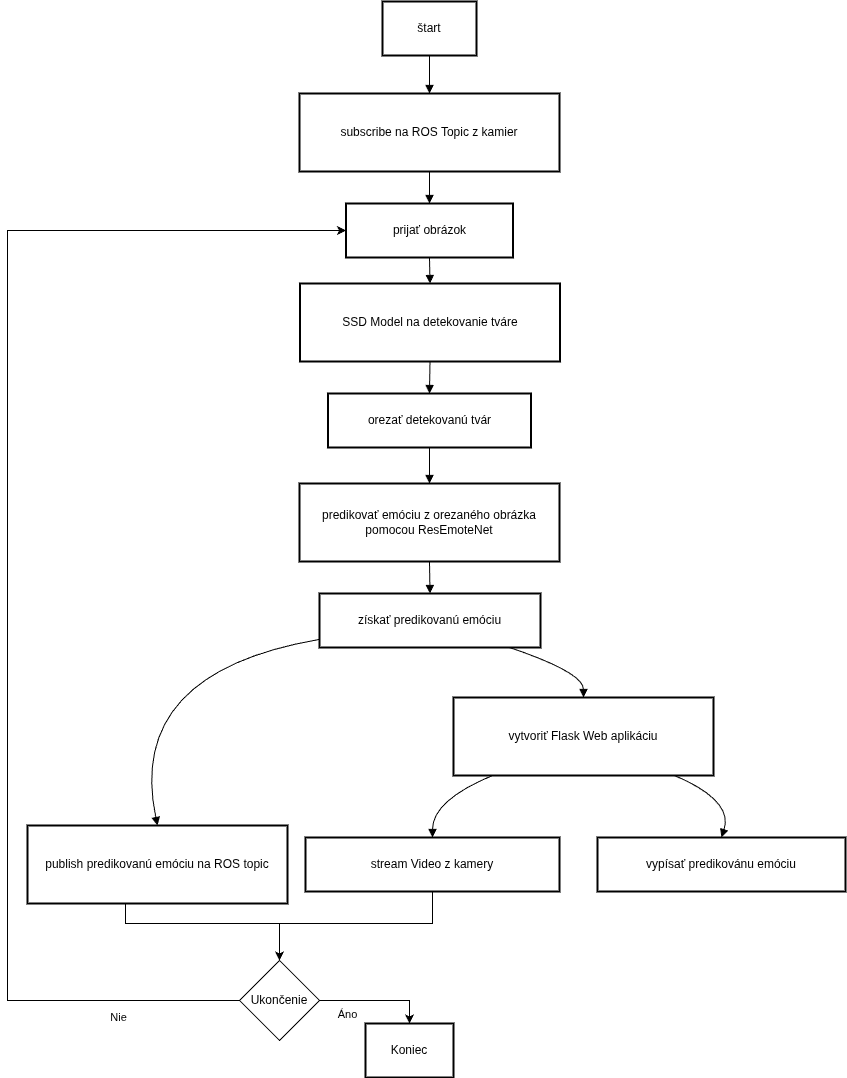
\includegraphics[width=0.8\textwidth]{img/predikovanie_diagram.png}
    \caption{Architektúra systému pre rozpoznávanie emócií v ROS2}
    \label{fig:ros2_architecture}
\end{figure}


\begin{itemize}
\item Publikovanie obrazových dát:
  \begin{itemize}
  \item \texttt{/rgb\_stream/ximea} (Ximea kamera)
  \item \texttt{/rgb\_stream/default} (USB kamera)
  \end{itemize}
\item Spracovacie uzly:
  \begin{itemize}
  \item Face Detection Node: MTCNN + SGG model
  \item Emotion Classifier: Načítanie ResEmoteNet modelu
  \item Result Publisher: \texttt{/emotion\_predicted}
  \end{itemize}
\end{itemize}
\begin{figure}[!htpb]
    \centering
    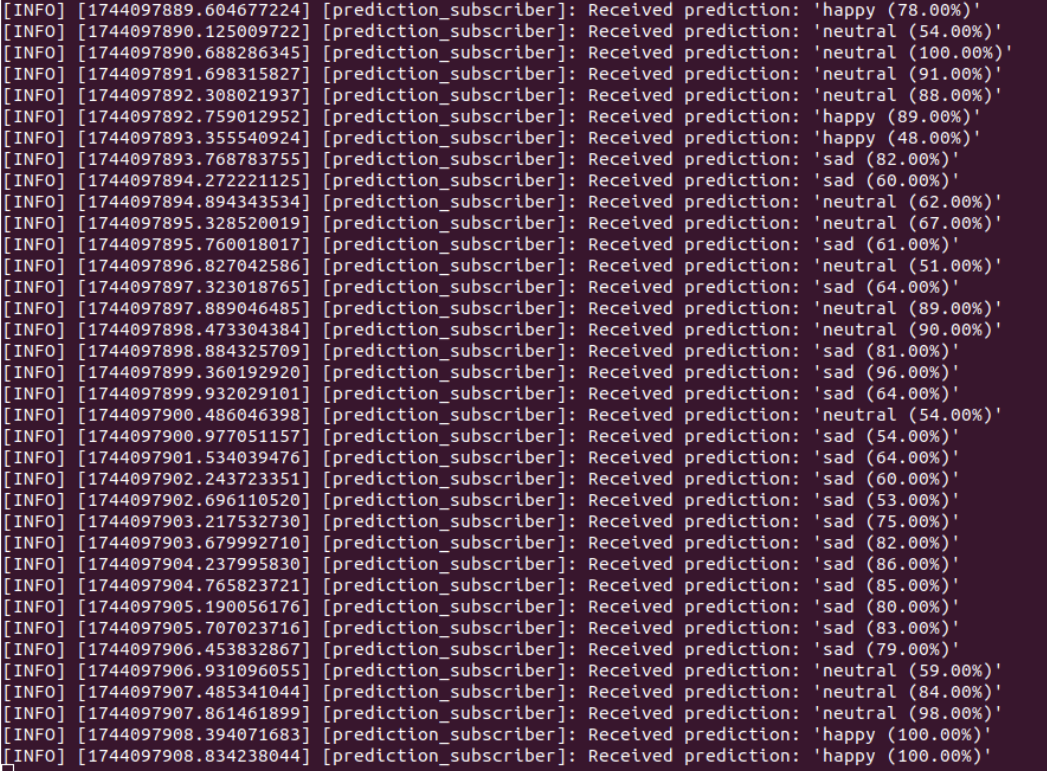
\includegraphics[width=0.7\textwidth]{img/subscriber.png}
    \caption{ROS subscriber na detekované emócie}
    \label{fig:ros2_architecture}
\end{figure}

\subsection{Webová vizualizácia pomocou Flask}
\begin{itemize}
\item Real-time stream s overlayom emočných štítkov
\item REST API pre konfiguráciu kamery a modelu
\item Integrácia s ROS2 cez \texttt{rosbridge\_server}
\end{itemize}

\begin{figure}[!htpb]
    \centering
    \begin{subfigure}{0.48\textwidth}
        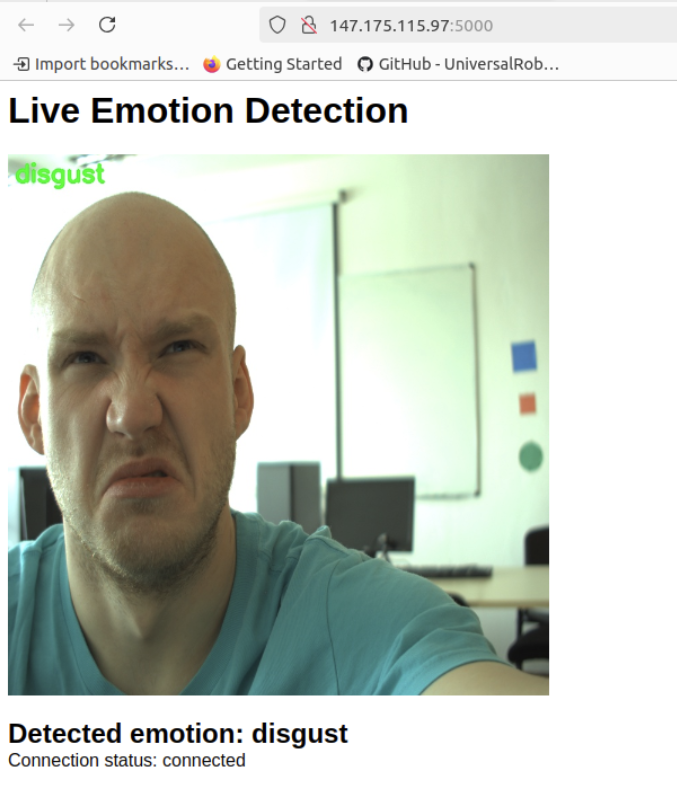
\includegraphics[width=\textwidth]{img/web_1.png}
        \caption{Webová vizualizácia výsledkov rozpoznávania emócií - znechutenie}
    \end{subfigure}
    \hfill
    \begin{subfigure}{0.48\textwidth}
        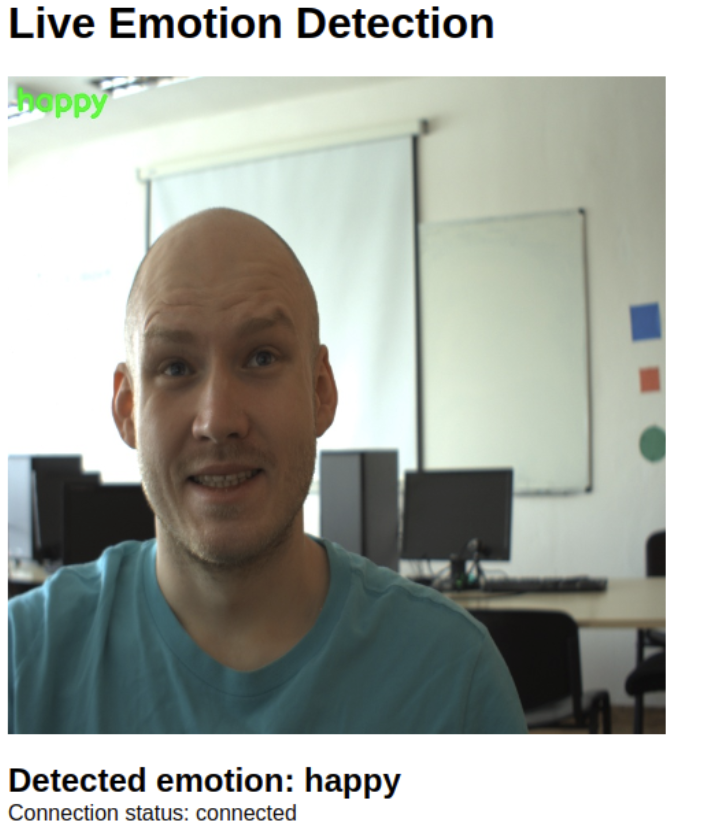
\includegraphics[width=\textwidth]{img/web_2.png}
        \caption{Webová vizualizácia výsledkov rozpoznávania emócií - šťastie}
    \end{subfigure}
    \caption{Príklady webovej vizualizácie systému pri testovaní na reálnych používateľoch}
    \label{fig:web_examples}
\end{figure}

\subsection{Validácia na robotickom pracovisku COCOHRIP}
    \begin{itemize}
\item Testovacia platforma URK FEI STU:
  \begin{itemize}
  \item Interakcia s robotom UR5e v reálnom čase
  \item Testovanie pri rôznych svetelných podmienkach
  \item Meranie latencie systému (500 ms)
  \end{itemize}
\end{itemize}

\subsection{Výsledky klasifikácie na datasete RAF-DB}
Model ResEmoteNet dosiahol nasledujúce presnosti pri klasifikácii jednotlivých emócií:
\begin{itemize}
    \item Šťastie: 94.76~\%
    \item Smútok: 89.32~\%
    \item Hnev: 87.45~\%
    \item Prekvapenie: 85.67~\%
    \item Strach: 83.12~\%
    \item Znechutenie: 81.45~\%
    \item Neutrálne: 95.23~\%
\end{itemize}

Výsledky ukazujú vysokú presnosť modelu pri rozpoznávaní výrazných emócií, zatiaľ čo jemnejšie prejavy ako strach a znechutenie dosahujú nižšiu presnosť.

\begin{figure}[!htpb]
    \centering
    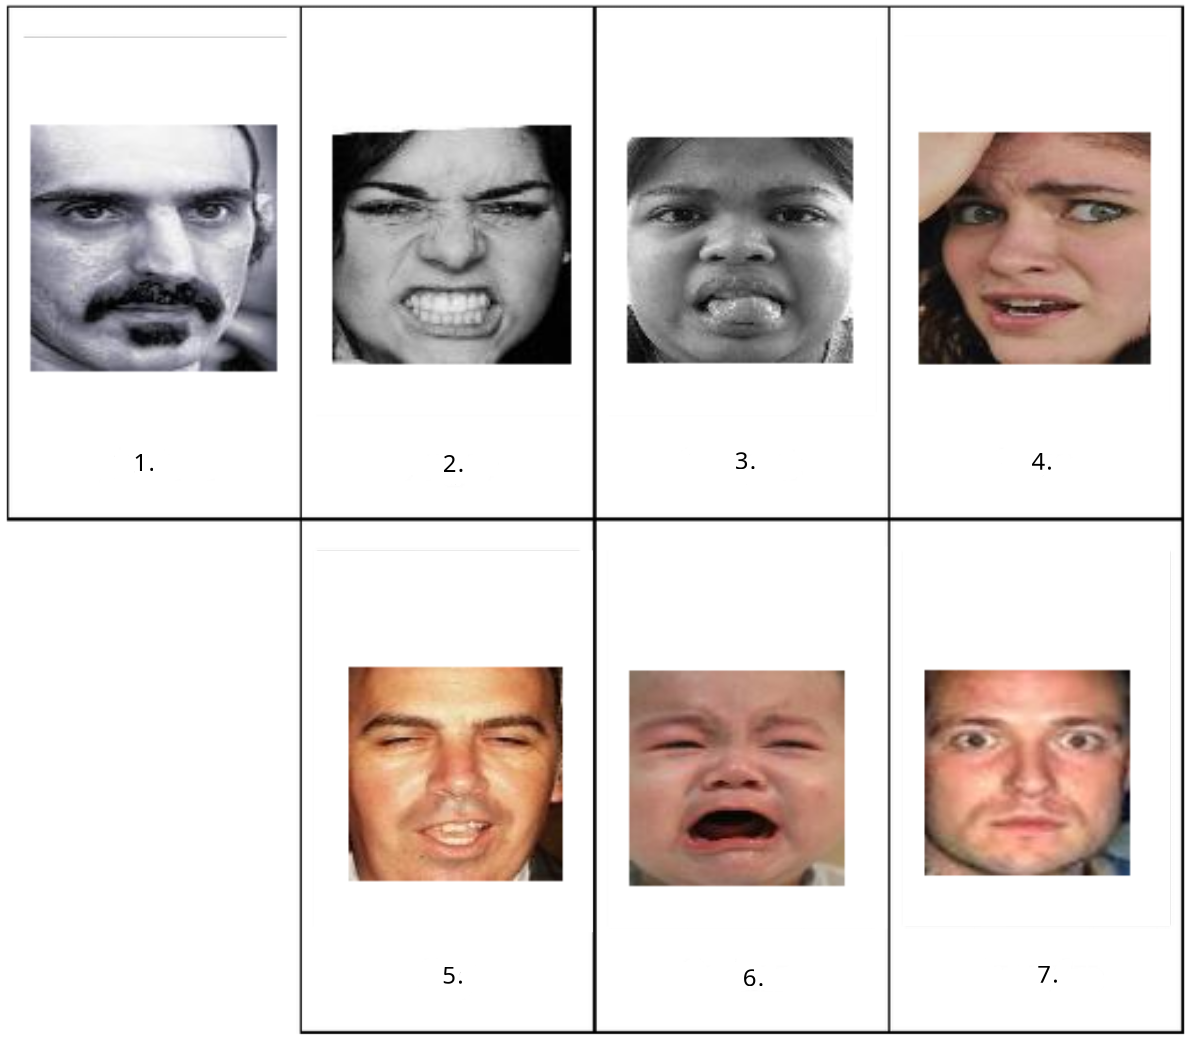
\includegraphics[width=0.8\textwidth]{img/emotions_dataset.png}
    \caption{Príklad obrázkov emócii z datasetu. 1. neutrálna, 2. hnev, 3. znechutenie, 4. strach, 5. šťastie, 6. smútenie, 7. prekvapenie \cite{li2017reliable}.} 
\end{figure}


\section{Exprerimenty a vyhodnotenie}
\label{sec:experiments}
\subsection{Úvod}
V tejto kapitole prezentujeme a analyzujeme experimenty, ktoré boli uskutočnené s cieľom overiť účinnosť navrhnutého systému na rozpoznávanie emócií na základe výrazu tváre. Systém bol testovaný nielen na otvorených datasetoch, ale aj v reálnych podmienkach, pričom sme overovali jeho správanie pri rôznych osvetleniach, na rôznych typoch kamier a v interakcii so skutočnými ľuďmi.

Jedným z hlavných cieľov experimentov bolo porovnať výkonnosť modelu so schopnosťami ľudských účastníkov pri identifikácii emócií z výrazu tváre. Na tento účel bol vytvorený dotazník, v ktorom respondenti označovali emócie na základe rovnakých vizuálnych vstupov, aké boli poskytnuté trénovanému modelu. Týmto spôsobom bolo možné objektívne porovnať rozdiely v úspešnosti medzi človekom a strojom.

Okrem dotazníkového experimentu sme tiež uskutočnili testovanie systému na reálnych zariadeniach. Testy prebiehali na rôznych kamerových platformách vrátane bežnej webkamery, kamery Azure Kinect a priemyselnej kamery Ximea. Zatiaľ čo rozdiely medzi jednotlivými kamerami boli minimálne, najväčší vplyv na presnosť predikcie mali svetelné podmienky. Zmeny v osvetlení, tieňovanie tváre alebo preexponovanie niektorých oblastí výrazne ovplyvňovali výsledky klasifikácie, čím sa potvrdila potreba robustných riešení schopných adaptácie na rôzne prostredia.

Nasledujúce podkapitoly detailne opisujú jednotlivé experimenty, prezentujú výsledky formou metrík a konfúznych matíc a poskytujú diskusiu o silných a slabých stránkach navrhnutého systému.
\subsection{Testovanie na re\'alnych d\'atach}

V r\'amci overenia praktickej pou\v{z}ite\v{l}nosti syst\'emu bolo vykonan\'e testovanie na re\'alnych \v{l}u\v{d}och v r\'oznych prostrediach a podmienkach. Cie\v{l}om tohto experimentu bolo zhodnoti\v{t}, ako si model porad\'i s predikciou em\'oci\'i v prostred\'i, ktor\'e sa l\'i\v{s}i od \v{s}tandardizovan\'ych datasetov pou\v{z}it\'ych po\v{c}as tr\'eningu.

\subsubsection{Priebeh testovania}
Experiment prebiehal v re\'alnom \v{c}ase na piatich \'u\v{c}astn\'ikoch, pri\v{c}om \'u\v{c}astn\'ici boli sn\'iman\'i kamerou po\v{c}as toho, ako vyjadrovali r\'ozne em\'ocie. Tieto em\'ocie boli preddefinovan\'e (napr. \v{s}\v{t}astie, sm\'utok, strach, hnev, znechutenie, prekvapenie, neutr\'alna em\'ocia), a \'u\v{c}astn\'ici sa ich sna\v{z}ili nasimulova\v{t} \v{c}o najvernej\v{s}ie. V\'ystupy z kamery boli n\'asledne spracovan\'e tr\'enovan\'ym modelom, ktor\'y okam\v{z}ite ur\v{c}il pravdepodobn\'u em\'ociu na z\'aklade aktu\'alneho v\'yrazu tv\'are.

\subsubsection{Probl\'emov\'e em\'ocie: strach a sm\'utok}
Po\v{c}as testovania sa uk\'azalo, \v{z}e najv\"a\v{c}\v{s}ie probl\'emy mal model (rovnako ako \v{l}udsk\'i hodnotitelia) s rozl\'i\v{s}en\'im medzi em\'ociami \textbf{strach} a \textbf{sm\'utok}. D\^ovodom je ich v\'yrazn\'a vizu\'alna podobnos\v{t}, najm\"a v oblasti o\v{c}\'i a obo\v{c}ia. Obidve em\'ocie s\'u \v{c}asto sprev\'adzan\'e stiahnut\'ym obo\v{c}\'im, zn\'i\v{z}enou aktivitou v oblasti \'ust a celkov\'ym poklesom v\'yrazu, \v{c}o sp\^osobuje ich z\'amenu. Navy\v{s}e, ak \'u\v{c}astn\'ici neprejavili em\'ociu dostato\v{c}ne intenz\'ivne, doch\'adzalo k nespr\'avnym klasifik\'aci\'am, ke\v{d} model vyhodnotil v\'yraz ako \textbf{neutr\'alny} alebo zamenil em\'ociu s najbli\v{z}\v{s}\'im vizu\'alnym prejavom.

\subsubsection{Pozorovania}
\begin{itemize}
    \item V pr\'ipade \textbf{strachu} sa \v{c}asto st\'avalo, \v{z}e model em\'ociu neklasifikoval spr\'avne, ak bola tv\'ar nedostato\v{c}ne nasvieten\'a. Jemn\'e znaky, ako roz\v{s}\'iren\'e o\v{c}i \v{c}i nap\"atie v tv\'ari, sa stratili pri slab\v{s}om osvetlen\'i.
    \item \textbf{Sm\'utok} bol niekedy rozpoznan\'y ako \textbf{znechutenie}, ak sa \'u\v{c}astn\'ikovi zvr\'asnila tv\'ar nevhodn\'ym sp\^osobom alebo bola kamera pr\'i\v{l}i\v{s} n\'izko.
    \item V niektor\'ych pr\'ipadoch sa prejavil rozdiel medzi \textbf{simulovanou} a \textbf{skuto\v{c}nou} em\'ociou -- model mal probl\'em rozpozna\v{t} \uv{nahran\'y} v\'yraz, ktor\'y neobsahoval typick\'e mikrov\'yrazy spojen\'e s danou n\'aladou.
\end{itemize}

\subsubsection{Zhrnutie}
Tento experiment uk\'azal, \v{z}e hoci model dosahuje velmi dobr\'e v\'ysledky v kontrolovan\'ych podmienkach, jeho v\'ykonnos\v{t} m\^o\v{z}e by\v{t} ovplyvnen\'a prirodzenos\v{t}ou v\'yrazu a sveteln\'ymi podmienkami. Preto je d\^ole\v{z}it\'e pri praktickom nasaden\'i po\v{c}\'ita\v{t} s mo\v{z}nos\v{t}ou ch\'yb pri em\'oci\'ach, ktor\'e s\'u vizu\'alne podobn\'e alebo subt\'ilne.

\textbf{Príklady z praxe.}

\subsection{Dotazn\'ikov\'y experiment s \v{l}u\v{d}mi}

V snahe porovna\v{t} schopnosti modelu s \v{l}udskou percepciou em\'oci\'i bol vytvoren\'y dotazn\'ik, v ktorom respondenti klasifikovali em\'ocie z\'obrazen\'e na rovnak\'ych vstupn\'ych fotografi\'ach, ak\'e boli predlo\v{z}en\'e modelu. Ka\v{z}d\'y respondent mal za \'ulohu priradi\v{t} jednu z preddefinovan\'ych em\'oci\'i (\v{s}\v{t}astie, sm\'utok, hnev, strach, znechutenie, prekvapenie, neutr\'alna) ku ka\v{z}dej fotografii.

\subsubsection{Zber a spracovanie odpoved\'i}
Dotazn\'ik bol vyplnen\'y 11 respondentmi, ktor\'i klasifikovali s\'erie 52 obrazov náhodne vybraných z datasetu. Ich odpovede boli analyzovan\'e a vyhodnotili sme individu\'alne presnosti a celkov\'y priemer. Celkov\'a priemern\'a \'uspe\v{s}nos\v{t} \v{l}ud\'i dosiahla \textbf{64.4\%}, s hodnoteniami medzi 55.8\% a 73.6\%.

\begin{figure}[!htpb]
\centering
    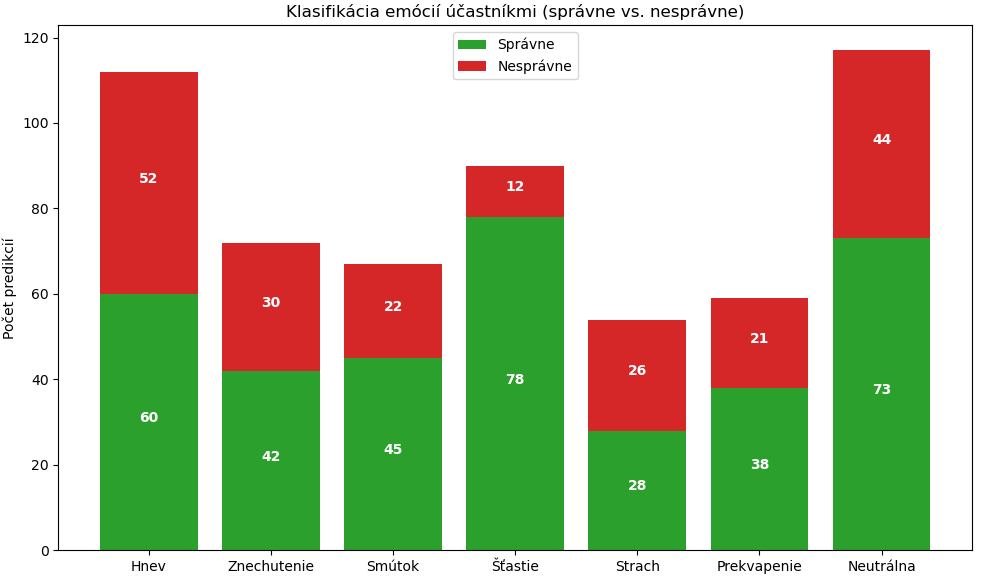
\includegraphics[width=0.8\textwidth]{img/experiments/google_form.png}
    % \title{Dotazn\'ik pre hodnotenie em\'oci\'i}
    \caption{Dotazn\'ik pre hodnotenie em\'oci\'i}
    \label{fig:google_form}
\end{figure}
\subsubsection{Naj\v{c}astej\v{s}ie chyby \v{l}ud\'i}
\begin{itemize}
    \item \textbf{Strach} bol \v{c}asto zamie\v{n}an\'y za \textbf{hnev}.
    \item \textbf{Prekvapenie} si respondenti \v{c}asto plietli so \textbf{neutr\'aln\'ym}.
\end{itemize}

\subsubsection{Porovnanie s modelom}
Model bol testovan\'y na rovnak\'ych vstupoch ako respondenti a dosiahol celkov\'u presnos\v{t} \textbf{90.4\%}. Zatia\v{l} \v{c}o \v{l}udia mali probl\'emy s niektor\'ymi em\'ociami, model vykazoval stabilne v\'ysledky s najv\"a\v{c}\v{s}ou chybovos\v{t}ou pri \textbf{prekvapen\'i} a \textbf{znechuten\'i}.
\begin{figure}[!htpb]
    \centering
    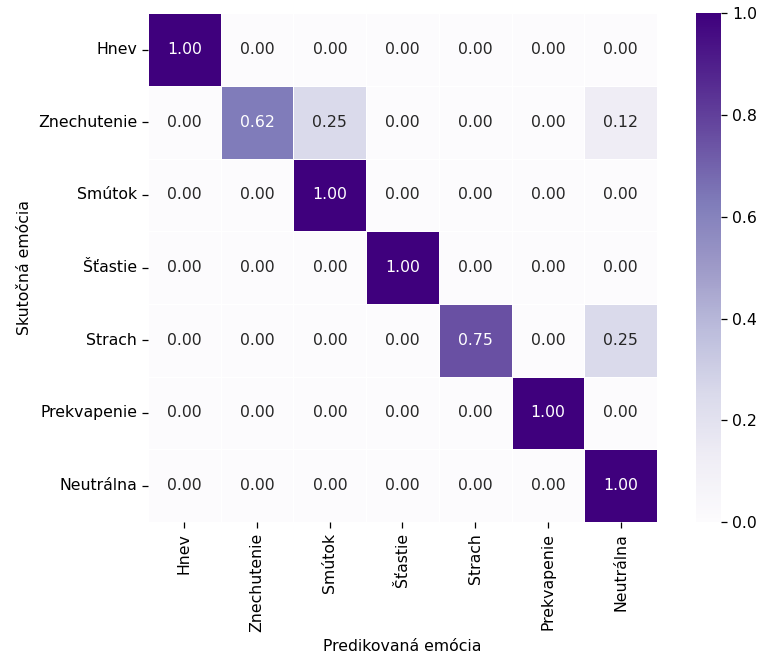
\includegraphics[width=0.8\textwidth]{img/experiments/confusion_nn_google_data.png}
    % \title{Dotazn\'ik pre hodnotenie em\'oci\'i}
    \caption{Neur\'ov\'a sie\v{t} s rovnak\'ymi vstupmi ako respondenti}
    \label{fig:nn_google_data}
\end{figure}
\subsection{Vizualiz\'acia v\'ysledkov}
\begin{itemize}
    \item Prilo\v{z}en\'a je konf\'uzna matica pre hodnotenia \v{l}ud\'i.
    \item Prilo\v{z}en\'a je konf\'uzna matica pre model.
    \item Graf porovn\'avaj\'uci priemern\'u presnos\v{t} \v{l}ud\'i a modelu.
\end{itemize}

\subsubsection{Zhrnutie}
Dotazn\'ikov\'y experiment uk\'azal, \v{z}e hoci \v{l}udia maj\'u schopnos\v{t} intuit\'ivne rozpozna\v{t} em\'ocie, model tr\'enovan\'y na rozsiahlych datasetoch dok\'aze dosahova\v{t} podstatne vy\v{s}\v{s}iu presnos\v{t}. Pri interpret\'acii em\'oci\'i m\^o\v{z}e by\v{t} rozhoduj\'uca konzistentnos\v{t} a pozornos\v{t} na detail, ktor\'e model zvl\'ada lep\v{s}ie ako n\'ahodn\'y respondent.

\subsection{Testovanie s r\'oznymi zariadeniami a podmienkami}

Na zhodnotenie robustnosti modelu bolo testovanie roz\v{s}\'{i}ren\'e o r\'ozne typy vstupn\'ych zariaden\'i a sveteln\'ych podmienok. Pou\v{z}it\'e boli viacer\'e kamery, konkr\'etne be\v{z}n\'a webkamera, kamera Azure Kinect a priemyseln\'a kamera Ximea.

\subsubsection{Výsledky na rôznych zariadeniach}
Pri testovan\'i na r\'oznych kamer\'ach boli zaznamenan\'e len minim\'alne rozdiely vo v\'ykone modelu. Presnos\v{t} klasifik\'acie zostala vysok\'a, \v{c}o potvrdzuje, \v{z}e model je schopn\'y efekt\'ivne pracova\v{t} s r\'oznymi typmi obrazov\'ych vstupov.

\subsubsection{Vplyv svetelných podmienok}
Najv\"a\v{c}\v{s}ie rozdiely boli pozorovan\'e pri zmene sveteln\'ych podmienok:
\begin{itemize}
    \item pri silnom alebo nehomog\'ennom osvetlen\'i bola z\'achytnos\v{t} mikrov\'yrazov zhor\v{s}en\'a,
    \item v pr\'ipade slab\'eho svetla alebo tie\v{n}ovania tv\'are sa zvy\v{s}ila chybovos\v{t}, najm\"a pri subtiln\'ych em\'oci\'ach ako strach alebo znechutenie,
    \item zmeny kontrastu a preexponovanie niektor\'ych \v{c}ast\\'i tv\'are viedli k chybn\'ym klasifik\'aci\'am.
\end{itemize}

\subsubsection{Zhrnutie}
Testovanie uk\'azalo, \v{z}e model je dostato\v{c}ne robustn\'y na r\'ozne hardv\'erov\'e konfigur\'acie, ale jeho v\'ykonnos\v{t} je citliv\'a na sveteln\'e podmienky. Preto je odpor\'u\v{c}an\'e pri praktickom nasaden\'i zabezpe\v{c}i\v{t} stabiln\'e a kvalitn\'e osvetlenie pri sn\'iman\'i tv\'are.

\subsection{Porovnanie s výsledkami modelu}

Porovnanie výstupov modelu a odpovedí ľudských účastníkov bolo realizované na identickej množine 52 snímok tvárí, ktoré zobrazovali jednotlivé základné emócie. Každý účastník dotazníka mal za úlohu priradiť jednej z týchto fotografií jednu z preddefinovaných emócií: radosť, smútok, hnev, strach, prekvapenie, znechutenie alebo neutrálny výraz. Tieto isté snímky boli následne spracované trénovaným modelom ResEmoteNet, čím bolo zabezpečené objektívne porovnanie medzi človekom a systémom.

Priemerná úspešnosť ľudských účastníkov dosiahla 64,4 \%, pričom jednotlivé výsledky sa pohybovali v rozmedzí od 55,8 \% do 73,6 \%. Naopak, model dosiahol presnosť 90,4 \%, čo poukazuje na jeho výrazne vyššiu konzistentnosť pri určovaní emócií.

Najvyššiu mieru zhody medzi človekom a modelom bolo možné pozorovať pri emócii radosť \ref{fig:happy_dataset}, ktorá bola ľahko rozpoznateľná vďaka charakteristickým znakom ako sú zdvihnuté kútiky úst a vrásky v oblasti očí. Neutrálny výraz bol správne klasifikovaný modelom vo väčšine prípadov, avšak u ľudí bol častejšie zamieňaný za mierne pozitívne alebo negatívne emócie.

\begin{figure}[!htpb]
    \centering
    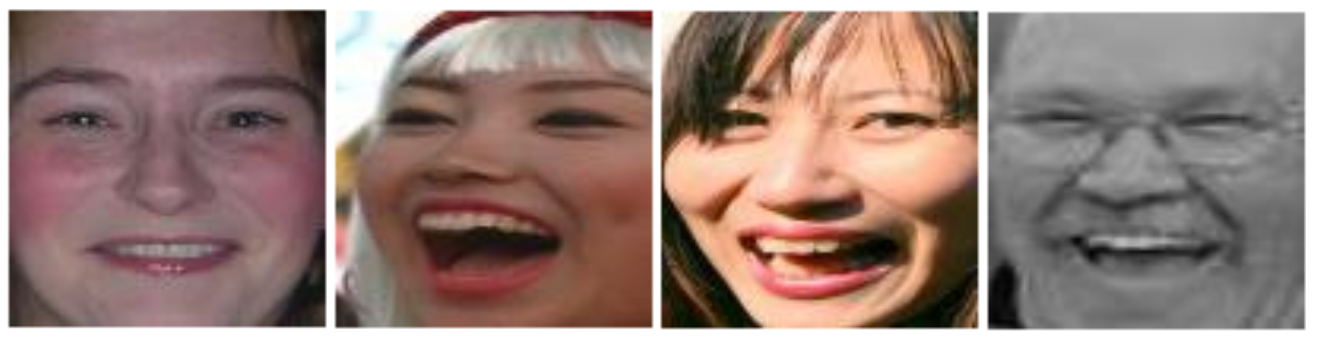
\includegraphics[width=0.65\textwidth]{img/stastny_dataset.png}
    \caption{Príklad emócie radosť z datasetu.}
    \label{fig:happy_dataset}
\end{figure}
\newpage
Rozdiely medzi modelom a respondentmi sa výraznejšie prejavili pri emóciách strach a znechutenie, na obrázku \ref{fig:mix_dataset} možno vidieť miernu podobu daných emócii. Tieto emócie boli zameniteľné aj medzi samotnými ľuďmi, čo naznačuje, že ich vizuálne prejavy sú menej jednoznačné a môžu sa prekrývať so smútkom alebo hnevom. Model v týchto prípadoch vykazoval vyššiu stabilitu v predikcii, no niekedy tiež dochádzalo k zámene s príbuznou emóciou.

\begin{figure}[!htpb]
    \centering
    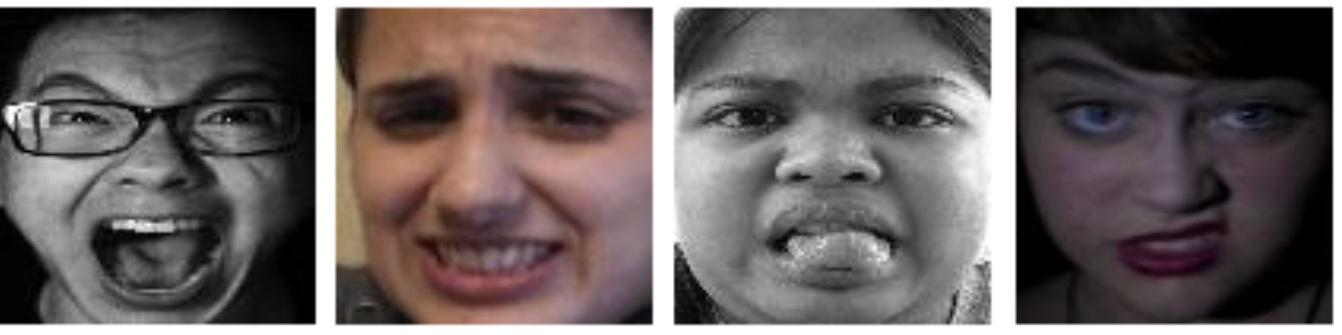
\includegraphics[width=0.65\textwidth]{img/mix_emotions.png}
    \caption{Príklad emócie strach, strach, znechutenie a znechutenie z datasetu.}
    \label{fig:mix_dataset}
\end{figure}
Výsledky taktiež ukázali, že niektorí respondenti mali tendenciu vyhodnocovať výrazy viac intuitívne, zatiaľ čo model pracoval výhradne na základe vizuálnych čŕt. Tento rozdiel v prístupe sa prejavil najmä pri výrazoch, ktoré boli menej výrazné alebo simulované bez silného emočného podkladu. V takých prípadoch sa stávalo, že ľudia reagovali odlišne než model – niekedy presnejšie, inokedy menej.

Celkovo možno konštatovať, že model dosahuje vyššiu presnosť ako priemerný ľudský hodnotiteľ, predovšetkým v kategóriách s dobre definovanými znakmi. Napriek tomu ľudia dokážu v niektorých prípadoch lepšie rozpoznať jemné nuansy a neverbálne signály, čo naznačuje, že spojenie oboch prístupov môže priniesť ešte spoľahlivejšie riešenia pre budúce aplikácie.

\subsection{Analýza výsledkov}

Výsledky experimentov ukázali, že model ResEmoteNet dosahuje vysokú presnosť pri rozpoznávaní emócií, najmä v kontrolovaných podmienkach s dobrým osvetlením a priamym pohľadom do kamery. Najspoľahlivejšie boli identifikované emócie radosť a neutrálny výraz, ktoré majú výrazné vizuálne znaky. Naopak, emócie ako strach a znechutenie boli častejšie zamieňané, a to aj medzi ľudskými hodnotiteľmi.

Dotazníkový experiment preukázal, že ľudia dosahovali priemernú úspešnosť okolo 64 \%, zatiaľ čo model vykazoval presnosť cez 90 \%, čo potvrdzuje jeho stabilitu. Zároveň sa ukázalo, že svetelné podmienky a prirodzenosť výrazu majú zásadný vplyv na presnosť rozpoznania, a preto je potrebné zabezpečiť kvalitné vstupné dáta.

Systém preukázal robustnosť voči rôznym kamerovým zariadeniam, no ostáva citlivý na nehomogénne alebo slabé osvetlenie. Výsledky potvrdili, že navrhnuté riešenie je vhodné na praktické použitie, pričom ďalšie zlepšenia možno dosiahnuť zapojením doplnkových modalít alebo využitím časového kontextu (napr. v podobe videa).

\subsection{Zhrnutie experimentov}

Experimenty preukázali, že navrhnutý systém na rozpoznávanie emócií na základe výrazu tváre je schopný spoľahlivo identifikovať základné emócie v reálnom čase a v rôznych podmienkach. Model \textit{ResEmoteNet} dosiahol vysokú presnosť najmä pri emóciách, ktoré majú jednoznačné vizuálne znaky – ako radosť, prekvapenie a neutrálny výraz. Porovnanie s výsledkami ľudských hodnotení potvrdilo, že model pracuje konzistentnejšie a s vyššou presnosťou ako priemerný človek.

\subsubsection{Silné stránky systému}
\begin{itemize}
  \item Vysoká presnosť klasifikácie v kontrolovaných podmienkach,
  \item Robustnosť voči typu použitej kamery (webkamera, RGB-D, priemyselná kamera),
  \item Reálne časové spracovanie obrazu a vhodnosť pre nasadenie v robotických systémoch,
  \item Výrazne lepšie výsledky oproti ľudským hodnotiteľom pri rovnakých vstupoch.
\end{itemize}

\subsubsection{Slabé stránky systému}
\begin{itemize}
  \item Zvýšená chybovosť pri zhoršených svetelných podmienkach a zakrytí častí tváre,
  \item Občasné zámene podobných emócií (napr. strach -- smútok, znechutenie -- hnev),
  \item Nízka spoľahlivosť pri simulovaných (neautentických) výrazoch bez prirodzených mikrovýrazov.
\end{itemize}

\subsubsection{Odporúčané metodológie a nástroje pre ďalší výskum}
\begin{itemize}
  \item Rozšírenie systému o multimodálne vstupy (napr. hlas, fyziologické signály),
  \item Zapojenie časového kontextu – využitie videosekvencií a modelov 3D CNN,
  \item Použitie adaptívneho osvetlenia alebo infračervených senzorov na elimináciu vplyvu svetelných podmienok,
  \item Experimentálne testovanie na väčšej vzorke účastníkov v prirodzených pracovných podmienkach (napr. pri reálnej interakcii človek--robot).
\end{itemize}

Z pohľadu praktického nasadenia je systém pripravený na integráciu do robotických platforiem, pričom jeho výkonnosť môže byť ďalej zlepšovaná kombináciou s ďalšími technológiami pre rozpoznávanie stavu operátora.

\section{Záver}
\label{sec:conclusion}
\subsection{Zhodnotenie práce}

Cieľom diplomovej práce bolo navrhnúť, implementovať a experimentálne overiť systém na rozpoznávanie emócií operátora na základe výrazu tváre. Tento cieľ bol úspešne naplnený prostredníctvom vytvorenia modulu využívajúceho model ResEmoteNet, ktorý bol trénovaný na dátach z reálnych databáz a integrovaný do robotického systému v prostredí \gls{ros}.

Navrhnutý systém dosahoval vysokú presnosť pri klasifikácii základných emócií, pričom najlepšie výsledky boli dosiahnuté pri kategóriách radosť, prekvapenie a neutrálny výraz. Systém bol úspešne otestovaný v rôznych podmienkach a s rôznymi typmi kamier, čo potvrdzuje jeho praktickú využiteľnosť v reálnom prostredí. V rámci dotazníkového experimentu bolo preukázané, že presnosť modelu je vyššia ako u bežných ľudských hodnotiteľov.

Z hľadiska zadania boli splnené všetky hlavné úlohy práce vrátane analýzy súčasných metód, návrhu architektúry systému, implementácie a testovania, ako aj vytvorenia samostatného \gls{ros} balíka pre jednoduchú integráciu. Výsledný systém predstavuje funkčné a rozšíriteľné riešenie, ktoré je možné nasadiť v rámci moderných kolaboratívnych robotických platforiem.

\subsection{Obmedzenia práce}

Aj napriek dosiahnutým pozitívnym výsledkom má navrhnutý systém niekoľko obmedzení, ktoré je potrebné zohľadniť pri jeho praktickom nasadení.

Jedným z hlavných obmedzení je citlivosť na svetelné podmienky. V prípade nehomogénneho alebo slabého osvetlenia môže dôjsť k zníženiu presnosti detekcie a klasifikácie emócií, najmä pri jemných alebo menej výrazných výrazoch tváre. Taktiež pri čiastočnom zakrytí tváre (napr. rukou, vlasmi alebo rúškom) sa výkonnosť modelu znižuje, čo je dôležité najmä v reálnych aplikáciách s nekontrolovaným prostredím.

Ďalším obmedzením je absencia časového kontextu – systém pracuje s jednotlivými snímkami bez zohľadnenia dynamiky výrazu tváre v čase. To obmedzuje jeho schopnosť rozpoznať prechodné alebo komplexnejšie emócie, ktoré sa prejavujú postupne.

Model bol trénovaný a testovaný na dátach z verejných datasetov a obmedzenej skupiny respondentov. Hoci výsledky naznačujú dobrú generalizáciu, pre úplnú robustnosť by bolo vhodné testovať systém na väčšom a diverzifikovanejšom súbore účastníkov, ako aj v rôznych pracovných scenároch.

Napokon, systém sa zameriava výlučne na vizuálnu modalitu, čím môže prísť o doplňujúce informácie z iných zdrojov, ako sú reč, tón hlasu alebo fyziologické parametre. Tieto vstupy by mohli zlepšiť presnosť a spoľahlivosť pri hodnotení emočného stavu operátora v komplexných situáciách.

\subsection{Budúce smerovanie}

Na základe identifikovaných obmedzení a získaných poznatkov z experimentov možno navrhnúť viacero smerov pre ďalší výskum a vývoj systému.

Jednou z hlavných oblastí rozšírenia je zapojenie ďalších modalít do procesu rozpoznávania emócií. Kombinácia vizuálnych údajov s rečou, tónom hlasu, pohybom tela by mohla zvýšiť presnosť a spoľahlivosť systému najmä v náročných podmienkach.

Ďalším prirodzeným krokom je spracovanie videosekvencií a zohľadnenie časového kontextu pomocou modelov ako 3D konvolučných sietí. Táto funkcionalita by umožnila identifikovať dynamiku výrazu tváre a mikrovýrazy, ktoré sú kľúčové pre rozpoznanie niektorých prechodných emócií.

V neposlednom rade je žiaduce realizovať dlhodobé testovanie v reálnom nasadení – napríklad v priemyselnom alebo zdravotníckom prostredí – kde sa dá overiť správanie systému v praxi, vrátane spätnej väzby od koncových používateľov. Takéto testovanie by poskytlo cenné poznatky pre ďalšiu iteráciu návrhu.

Rozšírenie systému týmto smerom prispeje k vytvoreniu komplexnejšieho a prirodzenejšieho spôsobu interakcie medzi človekom a robotickým systémom.
